% Master's thesis: maneuver-level traffic signal understanding.
% Build: tectonic main.tex, or latexmk -pdf main.tex (or upload the thesis/ folder to Overleaf, pdfLaTeX)
% Figures: python thesis/make_figures.py   (from the repository root)
\documentclass[12pt,a4paper,oneside]{report}

\usepackage[utf8]{inputenc}
\usepackage[T1]{fontenc}
\usepackage{lmodern}
\usepackage[english]{babel}
\usepackage{microtype}
\usepackage[a4paper,top=3cm,bottom=3cm,inner=3.5cm,outer=2.5cm]{geometry}
\usepackage{setspace}
\onehalfspacing

\usepackage{amsmath,amssymb}
\usepackage{graphicx}
\usepackage{booktabs}
\usepackage{tabularx}
\usepackage{multirow}
\usepackage{array}
\usepackage{xcolor}
\usepackage{caption}
\usepackage{subcaption}
\usepackage{enumitem}
\usepackage{listings}
\usepackage{tikz}
\usetikzlibrary{positioning,arrows.meta,fit,calc}
\usepackage{csquotes}
\usepackage[numbers,sort&compress]{natbib}
\usepackage[obeyspaces,spaces]{url}
\usepackage[hidelinks]{hyperref}
\usepackage[capitalise,noabbrev]{cleveref}

\graphicspath{{figures/}}
\captionsetup{font=small,labelfont=bf}
\setlist{itemsep=2pt,topsep=4pt}
\setlength{\emergencystretch}{3em}  % avoids overfull lines around long identifiers and citations
\lstset{basicstyle=\ttfamily\small,breaklines=true,frame=single,columns=fullflexible}

% Notation used throughout
\newcommand{\acccolor}{\mathrm{Acc}_{\mathrm{color}}}
\newcommand{\accpass}{\mathrm{Acc}_{\mathrm{pass}}}
\newcommand{\EM}{\mathrm{EM}}
\newcommand{\TSS}{\mathrm{TSS}}
\newcommand{\FG}{\mathrm{False\text{-}Go}}
\newcommand{\FS}{\mathrm{False\text{-}Stop}}
\newcommand{\dirs}{\mathcal{D}}
% Identifiers from the code base, breakable at _ . / | + and spaces
\DeclareUrlCommand\code{\urlstyle{tt}}
\makeatletter\g@addto@macro\UrlBreaks{\do\_\do\|\do\+}\makeatother
% Marks text the author still has to fill in or check
\newcommand{\todo}[1]{\textcolor{red}{[TODO: #1]}}
% Web references: a hand-written list (chapter "Web References"), cited as [W1], [W2], ...
\newcommand{\webcite}[1]{\ref{#1}}
\newcommand{\webitem}[1]{\item\label{#1}}

\begin{document}

\pagenumbering{roman}
\hypersetup{pageanchor=false}
% Replace this page with the official template of your university if one is required.
\begin{titlepage}
\centering
{\Large \textsc{\todo{University name}}\par}
\vspace{0.4cm}
{\large \todo{Faculty / Department}\par}
\vspace{0.2cm}
{\large \todo{Degree programme, e.g. Master's Degree in Computer Engineering}\par}

\vspace{2.5cm}
{\LARGE \bfseries Maneuver-Level Traffic Signal Understanding\\[0.2cm]
from a Single Front Camera:\\[0.2cm]
Replication, Structured Baselines and Cross-Dataset Robustness\par}

\vspace{2.5cm}
\begin{minipage}[t]{0.47\textwidth}
\raggedright
\textbf{Supervisor}\\
\todo{Prof. Name Surname}\\[0.4cm]
\textbf{Co-supervisor}\\
\todo{Name Surname (if applicable)}
\end{minipage}\hfill
\begin{minipage}[t]{0.47\textwidth}
\raggedleft
\textbf{Candidate}\\
Alessandro Contratto\\
Student ID: \todo{number}
\end{minipage}

\vfill
{\large Academic Year \todo{2025/2026}\par}
\end{titlepage}

\hypersetup{pageanchor=true}
\chapter*{Abstract}
\addcontentsline{toc}{chapter}{Abstract}

An automated vehicle approaching a signalized intersection does not need the color of every traffic
light in view; it needs to know whether its intended maneuver---straight, left or right---is
permitted. This thesis studies this \emph{maneuver-level} formulation of traffic signal understanding,
introduced by Zou et al., in which one front-camera image is mapped to a signal color and a stop/go
decision for each maneuver.

The work has three objectives. First, since the original benchmark is not public, it rebuilds the
maneuver-level labels from the lane and traffic-element topology of OpenLane-V2 and validates them
against the published label distribution. Second, it builds a structured model, in which a real-time
detector (RF-DETR) classifies each light by the maneuvers it controls and an explicit rule assigns colors
to maneuvers. Third, it tests transfer across countries, traffic rules and cameras, using new compatible
labels for the DriveU (Germany) and LISA (United States) traffic light datasets and a per-light
evaluation on ATLAS.

The rebuilt labels reproduce the published distribution for almost every class and indicate that the
original benchmark combines both OpenLane-V2 subsets under US rules. The structured model reaches a
Traffic Signal Score (TSS) of 0.899 on subset A and 0.915 on subset B, in the range published for the
end-to-end model. Trained on DTLD it reaches a test TSS of 0.958 at 22\,ms per frame; it transfers well
to LISA by day (0.952) but drops at night (0.863), and its False-Go rate doubles on Argoverse~2 images.
Right-turn signals, yellow lights, small distant lights and country-specific label conventions emerge
as the main open problems, and the safety-relevant errors concentrate exactly where aggregate metrics
do not look.

\vspace{0.5cm}
\noindent\textbf{Keywords:} traffic light recognition, autonomous driving, signal intent, DETR,
RF-DETR, OpenLane-V2, domain shift, traffic rules.


\tableofcontents
\listoffigures
\listoftables
\clearpage

\pagenumbering{arabic}
\chapter*{Introduction}
\addcontentsline{toc}{chapter}{Introduction}
\markboth{Introduction}{Introduction}

\section*{Context and motivation}

Signalized intersections are among the most demanding places for an automated vehicle. A single
junction can hold a dozen traffic lights: circular lamps for the main flow, arrow lamps for turning
lanes, lights for the opposite approach, lights of the next intersection further down the road and
pedestrian signals. A human driver resolves this scene almost instantly by knowing which lane they are
in, where they intend to go, and which lights are meant for them. For a perception system, the same
reasoning has to be made explicit.

Most traffic light recognition systems answer a narrower question: \emph{where} are the traffic
lights, and \emph{what color} is each one. Detecting and classifying lights is necessary, but it is not
what the planner consumes. The planner needs to know whether the maneuver it intends to perform is
permitted \emph{now}. Between the two questions lies a relevance and association problem---which of
the detected lights govern the ego vehicle, and which maneuver each of them controls---that has
traditionally been solved with prior high-definition (HD) maps storing the position of every light and
the lanes it serves~\cite{fairfield2011traffic,possatti2019traffic,polley2025atlas}. Maps are accurate
where they exist, but they are expensive to build and maintain and they fail silently when the world
changes. Map-free alternatives infer relevance from the image, using annotated lane
metadata~\cite{langenberg2019deep}, detected lane arrows~\cite{polley2024tldready} or a joint
detection and image-level classification model~\cite{trinci2026color}; they decide which lights are
relevant, but still not which maneuver each of them permits.

A recent line of work removes the map and asks the network to answer the planner's question directly.
Zou et al.~\cite{zou2026oneperception} formulate \emph{maneuver-level signal intent prediction}: from
one front-camera image, predict, for each of the four maneuvers straight, left, right and U-turn, the
color of the signal that governs it and whether the maneuver may proceed. (This thesis drops the U-turn,
which almost always follows the left-turn signal; \cref{sec:prob-def}.) Their direction-aware model
uses four learnable \emph{direction queries} that attend to a global image token and to region tokens
from an auxiliary traffic-light detector, and it outperforms both structured detection pipelines and
multimodal large language models on a benchmark derived from OpenLane-V2~\cite{wang2023openlanev2}.

\section*{Research problem}

The proposal is attractive but leaves several questions open. The benchmark labels and the code are not
released, so the reported numbers cannot be checked directly and the label semantics---which light
governs a maneuver, how a turn without its own arrow is treated---have to be reconstructed from the
paper. It is also unclear whether the end-to-end direction-query design is needed at all: the structured
pipelines it was compared with were designed for a different output, and a well-tuned modern detector
combined with a simple, explicit association rule might do as well. Finally, the evaluation is limited to OpenLane-V2,
which mixes US and Singapore driving under one set of rules. Traffic signals look different across
countries, and the rules that link a lamp to a maneuver differ too: in Germany a right turn obeys the
circular signal, while in the United States a right turn on red is generally permitted unless a
dedicated signal says otherwise~\cite{fhwa2009mutcd,stvo}. How a model trained in one setting behaves in
another is the question that matters most for deployment.

\section*{Objectives and research questions}

The thesis pursues three objectives:
\begin{enumerate}
  \item to \textbf{rebuild} the maneuver-level benchmark of Zou et al.\ from public data only,
        documenting every assumption that the reconstruction requires;
  \item to build and evaluate a \textbf{structured model} from a state-of-the-art real-time detector and
        the same label rules, under a statistically sound protocol;
  \item to \textbf{measure robustness} across datasets, countries, traffic rules, illumination and
        cameras.
\end{enumerate}
These objectives translate into three research questions:
\begin{description}[leftmargin=1.2cm,style=nextline]
  \item[RQ1] Can the benchmark labels be rebuilt from the public OpenLane-V2 annotations, and does the
             result match the published label distribution?
  \item[RQ2] How well does a structured pipeline, in which a detector predicts light classes that encode
             the controlled maneuvers and an explicit rule assigns them, solve the task, and where does
             it fail?
  \item[RQ3] How well does a model trained on one dataset transfer to others, and which conditions
             cause the largest degradation?
\end{description}

\section*{Methodology in brief}

The work is empirical. Per-frame, per-maneuver labels are derived from the lane graph and the
lane--traffic-element links of OpenLane-V2, for both its Argoverse~2 (subset A) and nuScenes (subset
B) parts, and the derivation is validated against the label distribution published by Zou et al.\
and by manual spot-checks. Compatible label builders are written for the DriveU Traffic Light Dataset
(DTLD)~\cite{fregin2018dtld} and the LISA Traffic Light Dataset~\cite{jensen2016vision}. Models are
trained on a single consumer GPU; all hyperparameters are tuned on a held-out part of the training
scenes so that the evaluation split is never used for model selection. Metrics follow the original
paper (color accuracy, passability accuracy, exact match, their mean TSS, and the False-Go and
False-Stop rates), and are complemented with per-direction analyses and a segment-level paired
bootstrap for comparisons between models.

\section*{Contributions}

\begin{itemize}
  \item An open reconstruction of the maneuver-level benchmark from OpenLane-V2, with documented rules
        whose output reproduces the published label distribution, and evidence that the benchmark
        combines subsets A and B under US driving rules.
  \item A structured RF-DETR model whose classes encode the maneuvers each light controls, so that a
        perfect detector reproduces every label, reaching a TSS of 0.899 on subset A and 0.915 on
        subset B of the rebuilt benchmark.
  \item Label builders for DTLD and LISA that follow the same conventions, a model trained on DTLD and
        an out-of-distribution evaluation on LISA, OpenLane-V2 and ATLAS.
  \item A per-direction error analysis showing where aggregate scores hide safety-relevant failures.
\end{itemize}

\section*{Structure of the thesis}

\Cref{ch:background} reviews traffic light recognition, the map-based, map-free and topology-based
approaches to deciding which lights are relevant, the maneuver-level formulation, the detection and
detection architectures used later, and the public traffic-light datasets. \Cref{ch:problem} analyses the maneuver-level task in depth: its formal definition,
the traffic rules behind the labels, the metrics and their blind spots, and the two design paradigms
for solving it. \Cref{ch:method} describes the data, the label construction, the model, the training
and evaluation protocol, and presents all results. \Cref{ch:discussion} discusses the findings against
the original paper and the literature, the limitations of the work and directions for future research.
The Conclusions summarize the answers to the research questions. The appendices collect the label
rules in detail, the full hyperparameters, per-epoch results and the commands needed to reproduce every
number.

\chapter{Theoretical Framework and Literature Review}
\label{ch:background}

This chapter introduces the concepts and the prior work on which the thesis builds. It starts from the
role of traffic signals in automated driving and the rules that give them meaning
(\cref{sec:bg-signals}). It then reviews traffic light recognition, from hand-crafted pipelines to
deep detectors (\cref{sec:bg-tlr}), and the central topic of this work: how a system decides
\emph{which} lights are relevant for the ego vehicle and which maneuvers they control
(\cref{sec:bg-relevance}). The detection and backbone architectures used later are covered in
\cref{sec:bg-detection,sec:bg-backbones}, the public datasets in \cref{sec:bg-datasets}, and the
chapter closes by positioning this work with respect to the literature (\cref{sec:bg-position}).

\section{Traffic signals in automated driving}
\label{sec:bg-signals}

Automated driving systems are commonly classified by the SAE J3016 levels of driving
automation~\cite{sae2021j3016}. From level~3 upwards the system, not the human, is responsible for
monitoring the environment within its operational design domain, so an urban system must interpret
traffic signals on its own. Vehicle-to-everything (V2X) communication could in principle broadcast
signal phases directly, but its deployment is still sparse, which leaves the camera as the only widely
available sensor for this task~\cite{polley2024tldready,polley2025atlas}. Unlike most other road
users, traffic signals carry no physical threat: their meaning is entirely conventional, defined by
national regulations that build on the 1968 Vienna Convention on Road Signs and
Signals~\cite{unece1968vienna}.

The conventions relevant to this thesis are those that link a lamp to a maneuver:
\begin{itemize}
  \item A \textbf{circular} lamp governs all maneuvers from the approach unless another signal
        overrides it. An \textbf{arrow} lamp governs only the maneuvers its arrow points to.
  \item In the \textbf{United States} the Manual on Uniform Traffic Control Devices
        (MUTCD)~\cite{fhwa2009mutcd} allows, in most jurisdictions, a right turn on a red circular
        signal after a full stop, unless a sign or a dedicated red right arrow prohibits it. A red
        circle therefore does not by itself stop a right turn.
  \item In \textbf{Germany} the Stra\ss enverkehrs-Ordnung (StVO)~\cite{stvo} makes the right turn
        obey the circular signal; turning right on red is allowed only where a green arrow sign
        (\emph{Gr\"unpfeil}) is mounted next to the light, and even then only after stopping.
  \item A \textbf{U-turn}, where legal, usually follows the left-turn signal; dedicated U-turn arrows
        are rare.
  \item The meaning of \textbf{yellow} differs: in Germany a red--yellow phase announces green, while in
        the United States yellow announces red.
\end{itemize}
The physical appearance of signals differs as well. European heads are mostly vertical three-lamp
housings mounted before the stop line, whereas US heads are often mounted on the far side of the
intersection, come in vertical and horizontal variants and are frequently seen from the back when
they serve the opposite approach~\cite{trinci2026color}. These differences are not cosmetic. A model
that learns ``right is free unless a right arrow is red'' or ``the largest light is the relevant one''
from data of one country will make wrong decisions in another. \Cref{ch:problem} returns to this point
when the label semantics are defined.

\section{Traffic light recognition}
\label{sec:bg-tlr}

Traffic light recognition (TLR) traditionally comprises the \emph{localization} of the lights in the
image and the \emph{classification} of their state (red, yellow, green, off) and, where present, of
their pictogram (circle or arrow direction).

\paragraph{Classical pipelines.} Early systems detected traffic lights with color segmentation in
suitable color spaces, followed by shape and blob analysis and temporal filtering. The survey of Jensen
et al.~\cite{jensen2016vision} reviews these approaches and identifies the problems that remain
relevant today: lights are small, their appearance depends strongly on exposure and on the camera, and
other light sources (tail lights, street lamps, reflections) look similar.

\paragraph{Deep detection.} With convolutional detectors, traffic lights became a standard, if
difficult, object detection problem; the survey of Pavlitska et al.~\cite{pavlitska2023survey} groups
the methods into adapted generic detectors, multi-stage pipelines (a detector followed by a state
classifier) and task-specific single-stage designs. Behrendt et al.~\cite{behrendt2017deep}
introduced the Bosch Small Traffic Lights Dataset together with a detection, tracking and
classification pipeline; Müller and Dietmayer~\cite{muller2018detecting} adapted single-shot detection
to the extreme aspect ratios and small sizes of lights.

\paragraph{Benchmarking across datasets.} Polley et al.\ (TLD-READY)~\cite{polley2024tldready} trained
YOLOv7, YOLOv8 and RT-DETR detectors on four datasets (BSTLD, LISA, DTLD and a private Karlsruhe set)
with a common protocol that evaluates on data unseen during training and keeps small and side-facing
lights in the test sets. For DTLD they extended YOLOv8 with the stride-4 feature level, to improve
small-light recall, and with two separate heads for state and pictogram. Their deployment on a research
vehicle exposed two weaknesses of public data: a model trained on DTLD reached only 0.28 mAP on frames
from the deployment camera (0.96 after fine-tuning on 9,000 annotated frames), and pictograms that no
public dataset contains, such as straight-right arrows, could not be recognized at all.

\paragraph{ATLAS.} The same group addressed these gaps with the ATLAS dataset and a complete
perception framework~\cite{polley2025atlas}. ATLAS annotates all vehicle lights in three time-synchronized
cameras of different focal length, covers every state--pictogram combination found in Germany
(including red--yellow and straight-right) and includes rain. A YOLO11 detector trained on DTLD and
ATLAS together keeps its DTLD accuracy while raising mAP@50 on the ATLAS test split from about 0.53 for
DTLD-only training to about 0.7, a direct measure of how far a single-camera dataset is from a
deployment setup. In the vehicle, one detector processes the medium camera and a second one alternates
between the tele camera (far lights) and the wide-angle camera (lights overhead at the stop line). The
framework is discussed further in \cref{sec:bg-maps}, since its relevance decisions come from an HD
map.

All these systems output light boxes with colors and pictograms. They leave open the question that the
planner actually needs answered: which of the lights matter for the ego vehicle, and for which
maneuver.

\section{Relevance: from lights to lanes and maneuvers}
\label{sec:bg-relevance}

A complex intersection can show a dozen lights at once, controlling different lanes, the opposite
approach or the next junction, and they frequently show different colors. Relevance estimation
decides which of them govern the ego vehicle. The literature offers four families of solutions, which
differ in the information they require at inference time; \cref{tab:relevance-methods} summarizes them.

\begin{table}[t]
\centering
\caption{Approaches to traffic light relevance. ``Inference input'' is what the method needs while
driving; ``Output'' is the granularity of the answer.}
\label{tab:relevance-methods}
\footnotesize
\begin{tabularx}{\textwidth}{@{}>{\raggedright\arraybackslash}p{3.0cm}>{\raggedright\arraybackslash}X>{\raggedright\arraybackslash}X>{\raggedright\arraybackslash}p{2.4cm}@{}}
\toprule
Method & Inference input & Output & Data \\
\midrule
Fairfield, Urmson~\cite{fairfield2011traffic} & image, prior 3D light map, localization & state of mapped lights & own \\
Possatti et al.~\cite{possatti2019traffic} & image, route-specific light map & stop/go of the route's lights & own \\
ATLAS framework~\cite{polley2025atlas} & two camera streams, HD map with signal groups & state per signal group & ATLAS \\
Langenberg et al.~\cite{langenberg2019deep} & image + lights, lane lines, lane arrows (annotated) & lights assigned to ego and neighbor lanes & DTLD + own labels \\
TLD-READY~\cite{polley2024tldready} & image (detected lights and road arrows) & relevant lights via arrow--pictogram matching & DTLD + own labels \\
Trinci et al.~\cite{trinci2026color} & image & per-light relevance and state; image-level stop/go/none & VZC-TLD, DTLD \\
TopoNet, TopoMLP~\cite{li2023graph,wu2024topomlp} & multi-camera images & lane graph and lane--light links & OpenLane-V2 \\
Zou et al.~\cite{zou2026oneperception} & front image & color and stop/go per maneuver & OpenLane-V2 \\
\bottomrule
\end{tabularx}
\end{table}

\subsection{Map-based relevance}
\label{sec:bg-maps}

Production-oriented systems sidestep most of the problem with prior maps. Fairfield and
Urmson~\cite{fairfield2011traffic} triangulate the 3D position of every light from mapping drives and
project it into the image during driving, enlarged to absorb localization errors, so that recognition
reduces to classifying the state of a small image region. Possatti et al.~\cite{possatti2019traffic}
combine a deep detector with a LiDAR-built map that stores only the lights relevant to the mapped
routes: detections outside the projected regions are discarded. The map makes relevance trivial, but
only for the route that was driven during mapping.

The ATLAS framework~\cite{polley2025atlas} is a modern instance of this family. Each detection is
back-projected as a 3D ray and matched to the mapped light positions by a minimum-cost bipartite
assignment (Hungarian algorithm~\cite{kuhn1955hungarian}) instead of a nearest-neighbor rule, which
makes the association robust to small calibration and localization errors. Lights that control the
same movement are grouped into \emph{signal groups}; a circular buffer per light accumulates
confidence-weighted detections over time, discounting old detections and those whose pictogram does
not match the map, and the most confident light of a group sets the group state. A relevant signal
group in an unknown state is conservatively treated as red. In 230 minutes of fully automated driving
in Karlsruhe the framework required no intervention, reached 99.3\% state accuracy within 120\,m and
reacted to phase changes in 184\,ms on average.

Maps solve both detection and relevance where they are accurate, but they must be built for every
intersection, kept current and localized against, and they fail silently when the infrastructure
changes. The remaining families try to infer relevance from the image itself.

\subsection{Map-free relevance estimation}

\paragraph{Heuristics.} The simplest map-free rules declare the largest, the topmost or the most
central light relevant. They are attractive because they need no training, but they fail whenever an
overhead light of another lane or the back of a far-side signal is more prominent than the ego lane's
light~\cite{polley2025atlas,trinci2026color}. Trinci et al.\ show that the largest-light rule works
reasonably on DTLD, where the relevant lights are usually the largest, but poorly on US data, where the
largest visible light is often irrelevant.

\paragraph{Traffic light to lane assignment.} Langenberg et al.~\cite{langenberg2019deep} formulate
relevance as traffic light to lane assignment (TL2LA): for the ego lane and its two neighbors, a CNN
predicts an \emph{indication vector} that marks the image columns of the lights assigned to that lane.
The image is down-sampled to $256\times256$ and its road part is warped to a bird's-eye view by
inverse perspective mapping. Their key idea is \emph{deep metadata fusion}: twelve binary metadata
feature maps (the boxes of all lights and of lights with particular arrow types, lane lines, lane
arrows, lane signs) are adaptively scaled and multiplied element-wise into an early convolutional layer. On 848
annotated DTLD sequences, fusion reaches about 93\% accuracy, more than rule-based, metadata-only and
vision-only alternatives and even above a group of 40 human raters on the full test set. The
limitation, pointed out by later work~\cite{polley2024tldready,polley2025atlas}, is that the metadata
are human annotations, which are not available while driving.

\paragraph{Lane arrows as relevance cues.} TLD-READY~\cite{polley2024tldready} replaces annotated
metadata with detections. A YOLOv8 model detects the directional arrows painted on the road, which are
larger and easier to see than the lights; a gradient-boosting classifier decides from each arrow's box,
class and offset from the image center whether it belongs to the ego lane; finally, the detected light
pictograms are matched to the relevant arrows (a right arrow to a right-arrow light or, if none
exists, to the circles). The method reaches 96\% relevance accuracy on DTLD without any map, but it
needs visible lane arrows, which disappear close to the stop line or under occlusion, and its tabular
relevance classifier did not transfer to the deployment camera without new labels. Code, weights and
the arrow-relevance labels for DTLD are public\,\webcite{web:tldready}.

\paragraph{Joint detection and relevance.} Trinci et al.~\cite{trinci2026color} argue that relevance
needs scene context that a plain detector does not capture, and solve a \emph{local} and a
\emph{global} task together. On a Faster R-CNN~\cite{ren2015faster} with a ResNet-50 backbone, two
extra heads predict the relevance and the state of each detected light from its pooled features
concatenated with its box coordinates. An image-level classifier then receives the feature pyramid
enriched with \emph{detection priors}, channels that are non-zero only where lights were detected, and
outputs one of three classes: relevant red (stop), relevant green (go) or no relevant light. Gradients
from the image-level classifier are stopped before the detection heads. Compared with heuristics, a
deep regression of the relevant light's position, RT-DETRv2 with relevance-aware classes, a Faster
R-CNN with attribute heads and a zero-shot vision--language model, the joint model is the most
accurate on both VZC-TLD and DTLD; removing the image-level classifier costs 5.8 points of image-level
mAP. Two findings are directly relevant here: images with \emph{no} relevant light are the hardest
class, because the model must recognize that \emph{all} visible lights are irrelevant, and models trained
on the German DTLD transfer poorly to the US VZC-TLD and vice versa.

\paragraph{Saliency-aware training.} Other works modify only the training signal. Greer et al.\ weight
the DETR loss towards salient (relevant) lights, which improves their recall but does not output a
relevance decision~\cite{greer2023salience}; Freitas et al.\ regress the image position where the
relevant light should appear~\cite{freitas2019relevant}.

\subsection{Topology reasoning}

The OpenLane-V2 benchmark~\cite{wang2023openlanev2} turned lane--traffic-element association into a
central task of driving-scene understanding. It annotates 3D lane centerlines, traffic elements in the
front image, and two topologies: lane-to-lane connectivity and lane-to-traffic-element links. Methods
such as TopoNet~\cite{li2023graph} and TopoMLP~\cite{wu2024topomlp}, and more recently
TopoPoint~\cite{fu2026topopoint} and one-stage designs that reuse attention maps as
topology~\cite{li2025reusing}, predict both graphs jointly from the camera images. A planner could
derive the permitted maneuvers from these graphs, but only after reconstructing the lanes and their
links correctly, so errors in any intermediate prediction propagate to the decision. This thesis uses
OpenLane-V2's annotated topology not as a prediction target but as the source from which maneuver-level
labels are derived.

\subsection{Maneuver-level signal intent}

Zou et al.~\cite{zou2026oneperception} take the last step and remove all intermediate
representations. Instead of light boxes, relevance flags or a graph from which the planner would still
have to infer what is allowed, they predict, for each of the four maneuvers straight, left, right and
U-turn, a color $c\in\{\text{none},\text{red},\text{yellow},\text{green}\}$ and a passability
$p\in\{\text{stop},\text{go}\}$. The task, called \emph{directional traffic signal understanding},
is posed on a benchmark derived from OpenLane-V2 by associating the annotated lights with ego
maneuvers through the lane topology. Its direction-aware model, described in detail in
\cref{sec:method-model}, uses a Swin Transformer backbone~\cite{liu2021swin} with an FPN, a lightweight
DETR-style light detector as auxiliary task, region-of-interest tokens of the detected lights, a global
image token and four learnable direction queries that attend to these tokens. The paper also defines
the evaluation protocol adopted in this thesis (color and passability accuracy, exact match, their
mean, the Traffic Signal Score, and the False-Go and False-Stop rates; \cref{sec:prob-metrics}).

The reported comparisons are three. Among generic backbones with plain classification heads, Swin-Tiny
is the strongest (TSS 0.873); adding the direction-aware design raises the TSS to 0.880 and lowers the
False-Go rate from 0.183 to 0.137. Multimodal large language models~\cite{liu2023visual}, which have
been applied to driving as visual question answering~\cite{sima2024drivelm}, stay behind even after
fine-tuning (TSS about 0.85--0.86 for 7--11B-parameter models) and fail almost completely zero-shot.
Finally, structured pipelines are clearly weaker: TLD-READY, adapted to the four-maneuver output with a
fallback to the approach's circular signal, reaches a TSS of 0.842 with a False-Go rate of 0.302, and
topology-based methods reach 0.66--0.71. The paper concludes that direct maneuver-level prediction is
more accurate and safer than multi-stage association. Neither the benchmark labels nor the code are
public. The present thesis replicates the best configuration of this work and revisits the comparison
with structured pipelines.

\section{Object detection}
\label{sec:bg-detection}

Both models studied in this thesis contain a detector, so the main detection paradigms are summarized
here.

\paragraph{Convolutional detectors.} Two-stage detectors such as Faster R-CNN~\cite{ren2015faster}
generate region proposals and classify pooled region features; the Feature Pyramid Network
(FPN)~\cite{lin2017feature} provides a multi-scale feature hierarchy that is particularly important for
small objects, and RoIAlign~\cite{he2017mask} extracts region features without quantization. One-stage
detectors such as YOLO~\cite{redmon2016you} predict boxes densely in a single pass and dominate
deployed traffic light detection~\cite{polley2024tldready,polley2025atlas}. Both families rely on
anchors or dense priors and on non-maximum suppression (NMS) to remove duplicates.

\paragraph{Detection transformers.} DETR~\cite{carion2020end} casts detection as set prediction: a
transformer decoder~\cite{vaswani2017attention} turns a fixed number of learned object queries into
boxes and classes, and training matches predictions to ground truth one-to-one with the Hungarian
algorithm~\cite{kuhn1955hungarian}. The matching cost and the loss combine a classification term, an
$L_1$ box term and the generalized IoU~\cite{rezatofighi2019generalized}. DETR removes anchors and NMS
but converges slowly. Deformable DETR~\cite{zhu2021deformable} replaces dense attention with sparse
sampling around reference points, which speeds up convergence and helps small objects; Group
DETR~\cite{chen2023group} accelerates training with several groups of queries, each matched
one-to-one.

\paragraph{Real-time detection transformers.} RT-DETR~\cite{zhao2024detrs} and
LW-DETR~\cite{chen2024lwdetr} showed that DETR-style detectors can match or beat YOLO-type detectors at
real-time speed, although earlier traffic light studies found RT-DETR weaker than YOLO on the small
lights of DTLD~\cite{polley2024tldready} and on relevance-aware classes~\cite{trinci2026color}.
RF-DETR~\cite{robinson2025rfdetr} builds on LW-DETR with a DINOv2~\cite{oquab2024dinov2}
self-supervised vision-transformer backbone and uses weight-sharing neural architecture search to
obtain a family of models (Nano to Large) that trade accuracy for latency; it is designed to be
fine-tuned on new domains. RF-DETR Medium is the detector of the structured baseline in this thesis.

\section{Image backbones}
\label{sec:bg-backbones}

Residual networks~\cite{he2016deep} pretrained on ImageNet~\cite{deng2009imagenet} were the default
backbone for a long time. The Vision Transformer~\cite{dosovitskiy2021image} applies a transformer to
image patches, but its global attention scales quadratically with resolution, which is a problem for
the high-resolution inputs that small traffic lights require. The \textbf{Swin
Transformer}~\cite{liu2021swin} restricts attention to local windows that shift between layers and
builds a four-stage hierarchy with strides 4 to 32, so it can serve as a drop-in replacement for
convolutional backbones in detection. \textbf{ConvNeXt}~\cite{liu2022convnet} modernized the
convolutional design along the same lines (large depthwise kernels, LayerNorm, inverted bottlenecks)
and matched Swin's accuracy; \textbf{ConvNeXt V2}~\cite{woo2023convnext} adds a global response
normalization (GRN) layer and fully convolutional masked-autoencoder (FCMAE) pretraining. Swin-Tiny and
ConvNeXt V2-Tiny have nearly the same size, channels and strides, which makes them a clean pair for an
ablation (\cref{sec:res-backbone}).

\section{Datasets}
\label{sec:bg-datasets}

Public data for traffic lights fall into two groups: dedicated traffic-light datasets, which annotate
lights in detail but rarely say which ones matter, and general driving datasets, in which lights are
one category among many. \Cref{tab:datasets} summarizes the datasets considered in this work; counts
refer to annotated images and vehicle-light boxes as distributed (or, where noted, as exported to the
common per-lamp format used here). Three properties determine how useful a dataset is for
maneuver-level prediction: whether it marks the \emph{relevant} lights, whether it annotates
\emph{pictograms} (arrows), and how diverse it is in country, camera and illumination.

\begin{table}[t]
\centering
\caption{Datasets considered in this thesis. St.\ = annotated states (R red, Y yellow, G green, O off,
U unknown); Pict.\ = arrow pictograms annotated; Relev.\ = how relevance is defined; Use = role in the
experiments (``--'' = surveyed only).}
\label{tab:datasets}
\footnotesize\setlength{\tabcolsep}{3pt}
\begin{tabularx}{\textwidth}{@{}llrrlllX@{}}
\toprule
Dataset & Region & Images & Lights & St. & Pict. & Relev. & Use \\
\midrule
LISA~\cite{jensen2016vision} & San Diego, US & 36k & 109k & RYG & left & -- & OOD test \\
BSTLD~\cite{behrendt2017deep} & California, US & 13k & 24k & RYGO & train & -- & -- \\
DTLD~\cite{fregin2018dtld} & Germany & 41k & 292k$^a$ & RYG+ & yes & route & train, test \\
S$^2$TLD~\cite{yang2022scrdet} & Shanghai, CN & 5.8k & 14k & RYGO & -- & -- & -- \\
VZC-TLD~\cite{trinci2026color} & US & 3.0k & 25k & RYGU & -- & lane & -- \\
ATLAS~\cite{polley2025atlas} & Karlsruhe, DE & 33k & 73k & RYG+ & yes & -- & OOD, per light \\
BDD100K~\cite{yu2020bdd100k} & US & 80k$^b$ & 213k$^b$ & RYG & -- & -- & -- \\
OLV2 A~\cite{wang2023openlanev2,wilson2021argoverse} & US & 27k$^c$ & -- & RYG & yes & topol. & train, eval \\
OLV2 B~\cite{wang2023openlanev2,caesar2020nuscenes} & US, SG & 34k$^c$ & -- & RYG & yes & topol. & train, eval \\
\bottomrule
\multicolumn{8}{@{}p{\textwidth}@{}}{\footnotesize RYG+: also red--yellow and off (DTLD also unknown).
$^a$ all lamp types, including pedestrian, bicycle and tram lights; $^b$ train and validation splits;
$^c$ front-camera frames of the train and validation splits. OLV2 = OpenLane-V2.} \\
\end{tabularx}
\end{table}

\subsection{Traffic-light datasets}

\paragraph{LISA.} The LISA Traffic Light Dataset~\cite{jensen2016vision}\,\webcite{web:lisa} was
recorded in San Diego and consists of day and night video sequences at $1280\times960$ pixels, about
36,000 annotated frames with 109,000 lights in total. Lights carry a state (red, yellow, green) and,
for some, a left or straight arrow, but no relevance information. Consecutive frames are highly
redundant, and the boxes are known to be loose and incomplete: some visible lights are not
annotated~\cite{polley2025atlas,fregin2018dtld}. Its night sequences, which make up more than half of
the test set, make it the main test of illumination robustness in this work.

\paragraph{Bosch Small Traffic Lights (BSTLD).} BSTLD~\cite{behrendt2017deep}\,\webcite{web:bstld}
contains about 13,400 images at $1280\times720$ recorded around Palo Alto, California, with about
24,000 annotated lights, many of them very small. The training split annotates 13 state--pictogram
classes; the test split only the four states red, yellow, green and off, which limits it to color
recognition. The test split is larger than the training split (8,334 versus 5,093 images).

\paragraph{DriveU Traffic Light Dataset (DTLD).} DTLD~\cite{fregin2018dtld}\,\webcite{web:dtld} is the
largest public traffic-light dataset: about 41,000 frames from 2,110 sequences in eleven German cities,
recorded at 1\,Hz with a stereo camera at $2048\times1024$ pixels and distributed as raw Bayer
images. It annotates about 292,000 lamps of all kinds with a rich attribute set: facing direction
(front, back, left, right), state (red, yellow, red--yellow, green, off, unknown), pictogram (circle,
left, right, straight and straight-left arrows, pedestrian, bicycle, tram), number of lamps, occlusion
and a \emph{relevant} flag. The flag marks the lights that serve the route the vehicle actually drove;
the route itself is not annotated, so a light can be irrelevant only because the vehicle went another
way. All sequences come from one vehicle and camera, mostly by day and in good weather, and each
sequence approaches a single intersection. DTLD is the training set for the German-rule models of this
thesis.

\paragraph{S$^2$TLD.} The SJTU Small Traffic Light Dataset~\cite{yang2022scrdet}\,\webcite{web:s2tld}
contains 5,786 images from Shanghai at $1920\times1080$ and $1280\times720$ with about 14,000 lights in
five classes (red, yellow, green, off and ``wait on''). It adds a Chinese urban
setting with very small lights but has neither pictograms nor relevance.

\paragraph{VZC-TLD.} The Verizon Connect Traffic Light Dataset~\cite{trinci2026color}\,\webcite{web:vzc}
contains about 3,000 dashcam images ($1280\times720$, 150° diagonal field of view) taken from 1,809
commercial vehicles of different sizes across the United States, each image from a different video
and thus a different intersection. Each of its 25,000 lights is annotated with a state (red, yellow,
green, unknown) and a binary relevance flag, defined as the light that governs the lane occupied by the
ego vehicle. It is small but far more diverse than DTLD in camera height, field of view, weather and
time of day, and it is the only public US dataset with relevance labels.

\paragraph{ATLAS.} The Applied Traffic Light Annotation Set~\cite{polley2025atlas}\,\webcite{web:atlas}
contains 33,044 images with 72,998 lights from three synchronized cameras of the research vehicle CoCar
NextGen in Karlsruhe: front-medium ($61^\circ\times39^\circ$, $1920\times1200$, 25,158 images),
front-tele ($31^\circ\times20^\circ$, $1920\times1200$, 5,109 images) and front-wide
($106^\circ\times92^\circ$, $2592\times2048$, 2,777 images). Lights are annotated from 2--4 pixels of
width, corresponding to distances of up to 200\,m on the tele camera, in 25 state--pictogram classes
that include all arrow combinations, red--yellow, off and two-lamp on-demand signals; 2,776 images were
recorded in medium to heavy rain. ATLAS provides no relevance or maneuver labels, so it is used here
only for a per-light evaluation of detection, color and arrow direction across cameras.

\subsection{Driving datasets with traffic-light annotations}

\paragraph{BDD100K.} BDD100K~\cite{yu2020bdd100k}\,\webcite{web:bdd100k} consists of 100,000 driving
videos crowd-sourced in several US regions, with one annotated key frame per video ($1280\times720$;
70,000 training, 10,000 validation and 20,000 test images). Among its object categories are traffic
lights with a color attribute; the training and validation splits together contain about 213,000 of
them. It covers a wide range of weather, times of day and cameras, but lights are often tiny and it has
neither pictograms nor relevance.

\paragraph{OpenLane-V2.} OpenLane-V2~\cite{wang2023openlanev2}\,\webcite{web:openlanev2} is built on
Argoverse~2~\cite{wilson2021argoverse} (subset A: seven ring cameras at 2\,Hz in six US cities; front
camera $1550\times2048$, portrait) and nuScenes~\cite{caesar2020nuscenes} (subset B: six cameras,
scenes in Boston and Singapore; front camera $1600\times900$). Traffic elements are annotated as 2D
boxes in the front image only, with an attribute that encodes the color for circular lights and the
direction for arrows. Its value for this thesis lies in the \code{topology_lcte} (lane centerline to
traffic element) and \code{topology_lclc} (lane to lane) annotations: together with the 3D centerline
geometry they make it possible to determine which maneuver each relevant light controls, so that
maneuver-level labels can be derived without manual annotation (\cref{sec:method-labels}).

\subsection{Use in this thesis}

OpenLane-V2 is the only dataset from which maneuver-level labels can be derived for every direction,
and it is the basis of the replicated benchmark. DTLD provides the second source of relevance---the
driven route---under German rules, and is used to train and test a model in a different country.
LISA and ATLAS, which lack relevance labels, serve as out-of-distribution test sets: LISA with
maneuver labels reconstructed from light sizes and kinds (US, day and night), ATLAS per light (Germany,
three cameras). BSTLD, S$^2$TLD, VZC-TLD and BDD100K were converted to the same per-lamp format but
are not used in the experiments reported here: they either lack the pictograms needed to tell which
maneuver a light controls, or, in the case of VZC-TLD, provide relevance only at the lane level. They
are natural candidates for the multi-dataset training discussed in \cref{sec:disc-future}.

The survey also shows a gap. Only three public sources say which lights matter, and each defines
relevance differently: by the route driven (DTLD), by the lane occupied (VZC-TLD) or by the annotated
lane topology (OpenLane-V2). None provides maneuver-level labels directly, and the two datasets with
pictograms and relevance (DTLD and OpenLane-V2) follow different national traffic rules.

\section{Positioning of this work}
\label{sec:bg-position}

The literature offers, on one side, mature light detectors that do not decide
relevance~\cite{behrendt2017deep,polley2024tldready} and, on the other, systems that decide relevance
with additional infrastructure or annotation: HD maps~\cite{fairfield2011traffic,polley2025atlas},
annotated lane metadata~\cite{langenberg2019deep} or predicted lane
topology~\cite{li2023graph,wu2024topomlp}. Map-free, image-only methods have so far produced a
per-light relevance flag or a single image-level stop/go decision~\cite{polley2024tldready,trinci2026color},
which does not distinguish between maneuvers. Maneuver-level prediction from a single
image~\cite{zou2026oneperception} answers the planner's question most directly, but it has been
evaluated on a single, unreleased benchmark, against structured baselines that were designed for a
different output, and in one traffic-rule setting only.

This thesis contributes an open reconstruction of that benchmark, an independent replication, a
comparison with a structured alternative whose classes are designed for the maneuver-level output, and
the first cross-dataset evaluation of the task that we are aware of, spanning US and German traffic
rules, day and night, and three camera fields of view.

\chapter{Maneuver-Level Signal Understanding: An In-Depth Analysis}
\label{ch:problem}

This chapter examines the task itself before any model is trained. It gives a formal definition
(\cref{sec:prob-def}), explains how the abstract notion of ``the signal that governs a maneuver'' is
made concrete in labels and why this depends on traffic rules (\cref{sec:prob-semantics}), discusses
the characteristics of the data that make the task hard (\cref{sec:prob-challenges}), analyses the
evaluation metrics and what they do not show (\cref{sec:prob-metrics}), and contrasts the two model
designs compared in this thesis (\cref{sec:prob-paradigms}).

\section{Task definition}
\label{sec:prob-def}

Let $I$ be a front-camera image and $\dirs=\{\text{straight},\text{left},\text{right}\}$
the set of maneuvers. The task is to predict, for every $d\in\dirs$,
\begin{align}
  c_d &\in \mathcal{C} = \{\text{none},\text{red},\text{yellow},\text{green}\}, \\
  p_d &\in \mathcal{P} = \{\text{stop},\text{go}\}.
\end{align}
The color $c_d$ is the state of the signal that governs maneuver $d$ for the ego vehicle at the next
intersection, or \emph{none} when no signal governs it. The passability is defined by the color through
the rule of Zou et al.\ (legend of their Fig.~2):
\begin{equation}
  p_d = \begin{cases} \text{stop} & \text{if } c_d = \text{red},\\ \text{go} & \text{otherwise.}\end{cases}
  \label{eq:pass-rule}
\end{equation}
Yellow therefore counts as \emph{go}, and so does \emph{none}: a maneuver without a governing signal is
not prohibited by a signal, even if other rules (yield, give way) apply. The model still predicts $p_d$
with a separate head, which the original paper motivates with the possibility of learning exceptions;
\cref{sec:res-perdir} shows that in practice the two outputs are almost perfectly coupled.

A frame-level label is the tuple $y = \big((c_d, p_d)\big)_{d\in\dirs}$. Since $p_d$ is a function of
$c_d$, the label space has $4^3=64$ possible states, of which far fewer occur in practice because
maneuvers are strongly correlated: straight and left share a signal whenever there is no dedicated left
arrow.

\paragraph{Why U-turn is left out.} Zou et al.\ define a fourth maneuver, the U-turn. This thesis drops
it. Dedicated U-turn signals are almost absent from the data, so a U-turn label takes the left signal in
99.9\% of the OpenLane-V2 frames, and DTLD and LISA have no U-turn signals at all. As a separate output,
U-turn therefore adds no information; it only counts the left turn a second time in every averaged
metric. All results in this thesis are computed over the three maneuvers, unless stated otherwise. The
paper's published numbers include U-turn, so comparisons with them are close but not exact. Removing
a near copy of left reweights the averaged metrics towards straight and right; since right is almost
always the trivial \emph{none} (\cref{sec:prob-metrics}), three-direction scores come out slightly
higher than four-direction scores of the same predictions.

\section{Label semantics and traffic rules}
\label{sec:prob-semantics}

The definition above hides the hardest part of the problem: deciding \emph{which} light governs a
maneuver. In OpenLane-V2 this has to be derived from the lane graph, and several choices have to be
made. The rules adopted in this thesis, detailed in \cref{sec:method-labels} and
\cref{app:labels}, follow a hierarchy of specificity:
\begin{enumerate}
  \item \textbf{Straight} takes the color of the lights that control the straight lane or that are
        generic (circular) lights of the approach.
  \item \textbf{Left} takes a left-specific light if one exists, and otherwise inherits the straight
        signal.
  \item \textbf{Right} takes only a \emph{dedicated} right-turn light; without one it is \emph{none}.
\end{enumerate}
The third rule encodes the US convention that a right turn on red is permitted
(\cref{sec:bg-signals}). It has two consequences that recur throughout the thesis. First, right is
\emph{none} in about 97\% of the OpenLane-V2 frames, so its color accuracy is dominated by a trivial
majority class. Second, the rare dedicated red right arrow, which is the one case where turning right
is actually forbidden, is extremely under-represented.

The convention also does not transfer. Under German rules (DTLD) the right turn obeys the circle when
there is no right arrow; applying the US rule there would declare most right turns unconstrained and
would be wrong. The DTLD labels in this thesis therefore use a second convention (\emph{signal}: right
takes a right arrow if present, otherwise the circle) and record it per frame, so that both training
and evaluation apply the correct rule. Right-turn labels thus mean different things across datasets,
which matters when models are evaluated out of distribution (\cref{sec:res-ood}).

A further subtlety concerns the left-hand traffic scenes of nuScenes (Singapore). A strict mirroring of
the rules (left becomes the near turn, right the far turn) would be the natural choice, but, as
shown in \cref{sec:res-labels}, it does not reproduce the label distribution of the original paper,
whereas applying US rules everywhere does. The replication therefore follows the US convention for
comparability, at the price of a known inconsistency: in Singapore a green right arrow yields
right~$=$~none.

\section{Characteristics and challenges of the data}
\label{sec:prob-challenges}

\paragraph{Small objects.} Traffic lights at the stop line of the next intersection are often 10--30
pixels tall in a 2048-pixel image, and they shrink by a factor of two to three when the image is
resized to a size a network can process. \Cref{sec:res-atlas} quantifies how strongly detection
recall depends on this height.

\paragraph{Relevance.} A frame can contain lights of the ego lane, of neighboring lanes with different
maneuvers, of the opposite approach (seen from the side), and of the next intersection. Lights of a far
intersection can have a different color from the near ones, and the label builder has to decide which
intersection is ``next''. When the most specific relevant lights disagree in color, the situation is
ambiguous and such frames are excluded from the benchmark.

\paragraph{Class imbalance.} Beyond the right-turn imbalance, yellow is rare (about 3\% of straight
labels) and short-lived, and \emph{none} for straight (T-junctions, turn-only lanes) is rare as well.
Rare classes carry little weight in pooled accuracy but include some of the most consequential
decisions.

\paragraph{Correlated frames.} The datasets consist of driving sequences sampled at 2\,Hz or more.
Consecutive frames usually show the same lights in the same state, so the effective number of
independent samples is closer to the number of intersection approaches than to the number of frames.
This has to be taken into account when comparing models statistically (\cref{sec:method-eval}).

\paragraph{Domain shift.} Lights differ in housing, size, mounting (overhead versus side poles) and
color rendition between countries and cameras; night images change their appearance completely; and
the camera geometry (portrait Argoverse~2 images, wide DTLD images, 4:3 LISA images) changes the scale
and aspect ratio at which lights appear after resizing.

\section{Evaluation metrics and their blind spots}
\label{sec:prob-metrics}

The metrics follow Eqs.~4--7 of Zou et al. For $N$ frames with predictions $\hat c_{i,d}$, $\hat
p_{i,d}$:
\begin{align}
  \acccolor &= \frac{1}{|\dirs|N}\sum_{i=1}^{N}\sum_{d\in\dirs} \mathbb{1}[\hat c_{i,d} = c_{i,d}], \\
  \accpass &= \frac{1}{|\dirs|N}\sum_{i=1}^{N}\sum_{d\in\dirs} \mathbb{1}[\hat p_{i,d} = p_{i,d}], \\
  \EM &= \frac{1}{N}\sum_{i=1}^{N} \prod_{d\in\dirs} \mathbb{1}[\hat c_{i,d}=c_{i,d} \wedge \hat p_{i,d}=p_{i,d}], \\
  \TSS &= \tfrac{1}{3}\left(\acccolor + \accpass + \EM\right),
\end{align}
and, pooling over frames and directions,
\begin{equation}
  \FG = P(\hat p = \text{go} \mid p = \text{stop}), \qquad \FS = P(\hat p = \text{stop} \mid p = \text{go}).
\end{equation}

The Traffic Signal Score (TSS) is a convenient single number, but it has properties worth making
explicit:
\begin{itemize}
  \item \textbf{Trivial directions inflate it.} Because right is \emph{none} in $\sim$97\% of frames, a
        model that never predicts anything else for right gains almost a third of $\acccolor$ and
        $\accpass$ for free. For this reason, out-of-distribution results are also reported without the
        right direction.
  \item \textbf{It is symmetric in the errors that matter asymmetrically.} Predicting \emph{go} for a
        red signal (False-Go) can cause a collision; predicting \emph{stop} for a green one (False-Stop)
        causes an unnecessary stop and possibly a rear-end risk, but is generally the safer failure.
        TSS weights both equally. The False-Go and False-Stop rates are therefore reported alongside.
  \item \textbf{Pooling hides directions.} False-Go is pooled over directions, so the rare
        right-turn stops barely influence it even if the model misses all of them. Per-direction
        results are necessary to see this.
  \item \textbf{Accuracy and passability are coupled.} Under \cref{eq:pass-rule}, $\accpass\ge\acccolor$
        whenever the predicted passability follows the predicted color, because some color errors
        (green vs yellow vs none) do not change passability.
\end{itemize}
To make the per-direction numbers interpretable, each is compared with a \emph{majority} baseline: the
accuracy of always predicting that direction's most frequent color.

\section{Two design paradigms}
\label{sec:prob-paradigms}

Two ways of solving the task are compared in this thesis.

\paragraph{End-to-end (direction-aware).} The network maps the image directly to the 3$\times$2
outputs. Relevance, association and traffic rules are learned implicitly from data. An auxiliary
detector supplies localized evidence, but its output is consumed as features, not as decisions. The
advantages are flexibility (context such as lane markings or road layout can be used without being
modeled) and a single training objective. The drawbacks are opacity---it is hard to know \emph{why} a
maneuver was declared free---and the fact that the traffic rules are baked into the weights: a change
of convention requires relabeling and retraining.

\paragraph{Structured (detector + rules).} A detector predicts, for each light, a class that encodes
both its color and the set of ego maneuvers it controls (for instance \code{left+straight|red}, or
\code{irrelevant|green} for lights of other lanes or junctions). A fixed rule then assigns colors to
maneuvers with the same specificity hierarchy used to build the labels. When the detector is perfect,
this pipeline reproduces every label exactly (an ``oracle'' property verified in
\cref{sec:method-rfdetr}), so all its errors are detection, classification and relevance errors. The
advantages are interpretability, the possibility of changing the rule at inference time (US versus
German right turns) and the reuse of mature detection architectures. The drawbacks are the larger,
sparser class space and the dependence on a score threshold.

The empirical comparison of the two paradigms is the subject of \cref{sec:res-rfdetr}.

\chapter{Research Methodology and Analysis}
\label{ch:method}

This chapter describes how the research was carried out and presents its results. The first half
covers the methodology: the overall design (\cref{sec:method-design}), the data and the construction
of labels (\cref{sec:method-labels}), the structured model and its training (\cref{sec:method-rfdetr})
and the evaluation protocol (\cref{sec:method-eval}). The second half reports the results in the order
of the research questions (\cref{sec:res-labels} to \cref{sec:res-cost}).

\section{Research design}
\label{sec:method-design}

The study is a quantitative, experimental one. The benchmark of Zou et al.\ is rebuilt from public
annotations, since neither its labels nor its code are released, and every quantity that the paper does
not specify is treated as a free design choice, made on the basis of standard practice or of tuning on
held-out training data, and documented. Three principles guided all experiments:
\begin{enumerate}
  \item \textbf{No model selection on evaluation data.} Hyperparameters, score thresholds and the
        number of epochs are chosen on a \emph{tune split} of 10\% of the training scenes. Where the
        evaluation split is the official validation set (OpenLane-V2), the reported model is the last
        completed epoch, not the best one.
  \item \textbf{Controlled comparisons.} Comparisons change one factor at a time (the training data, the
        evaluation domain), with everything else, including the random seed, fixed.
  \item \textbf{Verifiable components.} Label builders are unit-tested and checked by hand on frames
        with difficult configurations; the metrics are unit-tested; the structured model is checked
        with a ground-truth oracle.
\end{enumerate}

All experiments ran on a single NVIDIA RTX~5070 (12\,GB) with PyTorch~2.14.1~\webcite{web:pytorch}, CUDA~13.0 and
the \code{rfdetr} library~1.11.2~\webcite{web:rfdetr}. The code is organized as a Python package (\code{dtsu}) with tools for data export,
training, evaluation and visualization; \cref{app:repro} lists the commands that reproduce every
number in this chapter.

\section{Data and label construction}
\label{sec:method-labels}

\subsection{OpenLane-V2}

Both subsets of OpenLane-V2~\webcite{web:openlanev2} are used, front camera only: \code{ring_front_center} of Argoverse~2 for
subset A (1550$\times$2048, portrait) and \code{CAM_FRONT} of nuScenes for subset B
(1600$\times$900). Since only the front-camera images are needed, only those were extracted from the
image archives, which bundle all cameras. The official validation split serves as evaluation set, as in
the original paper; the official test split has no usable annotations.

\paragraph{Rules.} Per-frame, per-maneuver labels are built from four annotations: the lane-to-traffic
element links (\code{topology_lcte}), the lane-to-lane links (\code{topology_lclc}), the centerline
geometry, and the traffic-element attribute (1 red, 2 green, 3 yellow, 4--12 arrow types). The procedure
has four steps (full details in \cref{app:labels}):
\begin{enumerate}
  \item \textbf{Maneuver per lane.} Each lane is followed along its successors to the first junction
        lane being entered, which must start no more than 3\,m behind the ego vehicle. The heading change
        along that junction lane gives the maneuver: within $30^\circ$ straight, beyond $135^\circ$
        U-turn, otherwise left or right by sign. U-turn is kept at this step only so that a light
        controlling nothing but U-turn lanes is not mistaken for a left-turn light; it is not an output.
  \item \textbf{Relevant lights.} Lights linked to lanes that are aligned with the ego heading (within
        $60^\circ$) and belong to the nearest junction (within 10\,m) are kept. If the ego vehicle has
        already passed the stop line, approach lanes ending within 30\,m behind it are used instead.
  \item \textbf{Lights to maneuvers.} The specificity hierarchy of \cref{sec:prob-semantics} assigns
        colors to maneuvers. The most specific light wins; when equally specific lights disagree, the
        frame is marked as a conflict.
  \item \textbf{Frame filter.} A frame is kept if at least one relevant colored light exists and there
        is no conflict (596 frames were dropped as conflicts).
\end{enumerate}

\paragraph{Validation.} Thirty validation frames covering five difficult cases (turn arrows,
straight~$=$~none, dedicated right signals, crossing the junction, conflicts) were inspected by eye.
The check revealed one error, a vehicle standing exactly at the stop line being assigned to the next
junction, which the 3\,m tolerance of step~1 corrects; all other inspected labels were correct or
plausible. \Cref{fig:examples} shows two labeled frames, and \cref{sec:res-labels} compares the
resulting distribution with the original paper.

\begin{table}[t]
\centering
\caption{Kept frames per split after label construction (OpenLane-V2, front camera).}
\label{tab:kept-frames}
\begin{tabular}{@{}lrr@{}}
\toprule
 & train & val \\
\midrule
Subset A & 10,141 / 22,477 & 2,220 / 4,806 \\
Subset B & 6,806 / 27,968 & 1,565 / 6,019 \\
A+B (this work) & 16,947 & 3,785 \\
Zou et al.~\cite{zou2026oneperception} & 23,904 & 5,147 \\
\bottomrule
\end{tabular}
\end{table}

\paragraph{Data scope.} The paper describes its benchmark as Subset-A, yet its frame counts (23,904
train, 5,147 val) exceed the total number of subset A frames \emph{before} any filtering (22,477 and
4,806). The paper's benchmark therefore cannot be subset A alone. Combining A and B fits its counts
better, and, as shown in \cref{sec:res-labels}, also its label distribution. All OpenLane-V2 models are
therefore trained on A+B and evaluated on subset A validation (the paper's reference set), subset B
validation and their union. \Cref{tab:kept-frames} lists the kept frames: this work keeps about 71\% as
many frames as the paper. The remaining difference cannot be resolved, since the paper's filtering
rules are not specified and it also applied manual quality control.

\paragraph{Tune split.} 10\% of the training scenes (70 per subset; 1,185 kept frames of A and 785 of
B) are held out as tune split. All hyperparameter decisions on OpenLane-V2 are made on it.

\subsection{DTLD and LISA}

Two further label builders produce records in the same format, so that datasets can be mixed and models
evaluated across them.

\paragraph{DTLD.} DTLD's \emph{relevant} flag marks lamps serving the route actually driven, which is
itself not annotated. The lamps serving each possible route are therefore re-derived from the
front-facing vehicle lamps at the ego intersection: a route with its own arrow is served by that arrow,
a route without one by the circles. Red--yellow (``prepare to go'') counts as red, since it still means
stop. Right turns follow the German rule (right arrow if present, otherwise the circle), recorded as
\code{near_turn = "signal"}; under this rule the training labels for right are 63\% green, 27\% red, 3\%
yellow and 7\% none, against 97\% none under the US convention. Frames are dropped for conflicting
lamps (619 in train), lamps that are off or of unknown state (656), disagreement with a reviewed
route-label rule (484), or the absence of a relevant vehicle lamp (949).

\paragraph{LISA.} LISA provides no relevance information. Lights at the ego intersection are identified
by size: a light is kept if it is at least 0.6 times as tall as the tallest light \emph{of the same
kind} (circle, left arrow, straight arrow). Comparing within a kind keeps far-side circles that would
otherwise be discarded next to a large near-side left-arrow pole, a case found during spot-checking.
Frames are dropped for conflicts (130 in train) and when only arrows are visible, because LISA leaves
some visible circles unannotated. Right is always \emph{none} under the US rule, since LISA has no
dedicated right-turn lights.

About 50 frames across both datasets were spot-checked on the same difficult cases as for OpenLane-V2.
Splits are listed in \cref{tab:ext-splits}: the official test sets are used for testing and a
validation split is held out from the official training data by whole sessions or clips.

\begin{table}[t]
\centering
\caption{Kept frames of the additional datasets. Images are resized to the canvas shown.}
\label{tab:ext-splits}
\begin{tabular}{@{}lrrrl@{}}
\toprule
 & train (fit) & val (tune) & test & canvas \\
\midrule
DTLD & 23,222 & 2,706 & 11,347 & 1024$\times$512 \\
LISA & 16,240 & 1,431 & 17,612 & 1024$\times$768 \\
\bottomrule
\end{tabular}
\end{table}

\section{The structured model}
\label{sec:method-rfdetr}

The model follows the structured paradigm of \cref{sec:prob-paradigms}: a detector classifies every
light by its color and by the ego maneuvers it controls, and an explicit rule turns the detections into
per-maneuver decisions.

\paragraph{Class encoding.} Every annotated light becomes one detection class \code{<moves>|<color>},
where \code{<moves>} is the set of ego maneuvers the light controls according to the label builder
(e.g.\ \code{left+straight}, \code{generic} for a circular light of the approach) or \code{irrelevant}
for lights of other lanes or junctions. On OpenLane-V2 A+B this gives 46 classes; on DTLD, whose
pictograms map to fewer combinations, 24.

\paragraph{Assignment rule.} At inference, detections above a score threshold are de-duplicated with
class-agnostic NMS (IoU 0.5) and their \code{<moves>} sets are passed to the same specificity hierarchy
used for the labels, with the highest score breaking ties between equally specific lights. The rule
takes the traffic convention as a parameter (US \emph{dedicated} or German \emph{signal} right turns).
Feeding ground-truth boxes through this rule reproduces every training label exactly (oracle TSS
$=1.0000$ on OpenLane-V2 and on DTLD fit, tune and test), so the model's errors are entirely due to
detection, classification and relevance.

\paragraph{Detector and training.} RF-DETR Medium (34.6M parameters) is fine-tuned from its released
detection-pretrained weights with the library's own recipe~\webcite{web:rfdetr} (optimizer, EMA, losses, schedule) except where it would corrupt
the labels: horizontal flips and random crops are disabled (a crop can remove the light that sets a
direction's label), multi-scale training is disabled in favor of a single square resolution of 1024
pixels, and brightness and contrast jitter is added (hue shifts are excluded because they change light
colors). The batch size is 4 with 4 gradient-accumulation steps. The complete settings are collected in
\cref{app:hparams} (\cref{tab:hparams-rfdetr}).

\paragraph{Tuning.} All model selection in this thesis (hyperparameters, epochs, score thresholds) was
done with four-direction scores, before U-turn was dropped; the selections are kept as they were made,
and the tune scores quoted for them are four-direction scores. On the tune split, RF-DETR Medium with
the default learning rate (tune TSS 0.905)
was better than Medium with half the learning rate (0.893) and than Large (0.896), and its tune TSS
plateaued after two epochs with a best score threshold of 0.20. The final model was trained for four
epochs on the full A+B training set with this threshold fixed, and the last epoch is reported; its
per-epoch results are listed in \cref{app:epochs} (\cref{tab:rfdetr-epochs}).

\paragraph{DTLD model.} The same recipe was trained on DTLD's fit split for 15 epochs, with a per-epoch
overfitting report: the eval-mode detection loss and the direction metrics on the held-out tune split
are compared with those on a fixed 1,000-frame probe of the training data. The tune split picks both
the epoch and the score threshold; DTLD test is only reported.

\section{Evaluation protocol}
\label{sec:method-eval}

All six metrics of \cref{sec:prob-metrics} are computed by one unit-tested function. Per-direction
results report $\acccolor$, $\accpass$, False-Go, False-Stop, the number of stop labels and the majority
baseline.

\paragraph{Statistical comparison.} Frames of the same driving segment are strongly correlated, so a
frame-level test would overstate the evidence. Two models are compared with a \emph{paired,
segment-level bootstrap}~\cite{efron1993introduction}: whole segments are resampled with replacement
(separately for the 112 segments of subset A val and the 65 of subset B val), both models are scored on
the same resample, and 10,000 resamples give a 95\% percentile interval and a two-sided p-value for the
difference of each metric.

\paragraph{Out-of-distribution evaluation.} A model trained on one dataset is scored on another only
after a label oracle check: every ground-truth light of the target is mapped to the model's class names
and pushed through the assignment rule with the target's traffic convention, and frames whose labels
cannot be reproduced this way are left out and counted (none of LISA; 1 of 2,220 frames of subset A
val). Any remaining gap is thus due to the detector. Results are given at two thresholds---the one
picked on the source tune split (the honest out-of-distribution number) and the best one on the
target's tune split (to measure how much of the gap is miscalibration)---and with two geometries:
squeezing the image to the square input, or first padding it to the 2:1 aspect ratio of the training
images.

% ---------------------------------------------------------------------------------------------------
\section{Results: label reconstruction}
\label{sec:res-labels}

\Cref{fig:label-dist} and \cref{tab:label-dist} compare the per-direction color distribution of the
reconstructed labels (A+B, train and val, kept frames) with Fig.~3 of the original paper.

\begin{figure}[t]
\centering
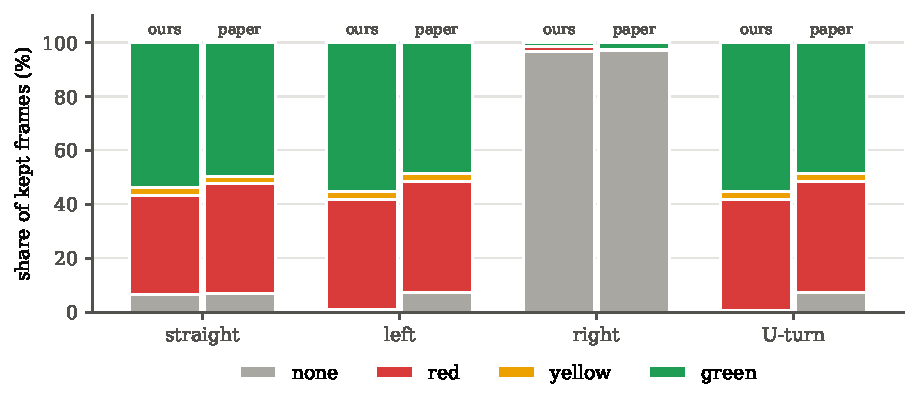
\includegraphics[width=\textwidth]{label_distribution.pdf}
\caption{Per-direction color distribution of the reconstructed labels (left bar of each pair) and of the
original benchmark (right bar, from Fig.~3 of Zou et al.).}
\label{fig:label-dist}
\end{figure}

\begin{table}[t]
\centering
\caption{Label distribution in \%, this work / Zou et al.\ (A+B, train + val, kept frames).}
\label{tab:label-dist}
\begin{tabular}{@{}lcccc@{}}
\toprule
Direction & none & red & green & yellow \\
\midrule
straight & 6.5 / 7.0 & 36.9 / 40.7 & 53.9 / 49.7 & 2.7 / 2.5 \\
left & 0.9 / 7.2 & 40.8 / 41.3 & 55.5 / 48.8 & 2.9 / 2.8 \\
right & 96.6 / 96.9 & 1.8 / 0.3 & 1.5 / 2.7 & 0.1 / 0.2 \\
\bottomrule
\end{tabular}
\end{table}

The distributions agree closely for straight and right, and for the colored classes of left. The
paper's Fig.~3 also shows U-turn, with a distribution nearly identical to left's; in the labels rebuilt
here U-turn takes the left signal in 99.9\% of the frames, which is why it is not used as a maneuver in
this thesis (\cref{sec:prob-def}). Two
observations support the reading that the original benchmark is A+B under US rules: subset A alone is
much greener (straight 28\% red, 64\% green), and mirroring the rules for the left-hand traffic scenes
of Singapore gives right~$=$~none in only 85.7\% of frames, far from the paper's 96.9\%. The one clear
mismatch is \emph{none} for left (0.9\% here, 7.2\% in the paper): in the paper, left
\emph{none} is about as frequent as straight \emph{none}, which suggests that its left labels inherit a
straight \emph{none} more often than the rules adopted here do.

\begin{figure}[t]
\centering
\begin{subfigure}[b]{0.36\textwidth}
  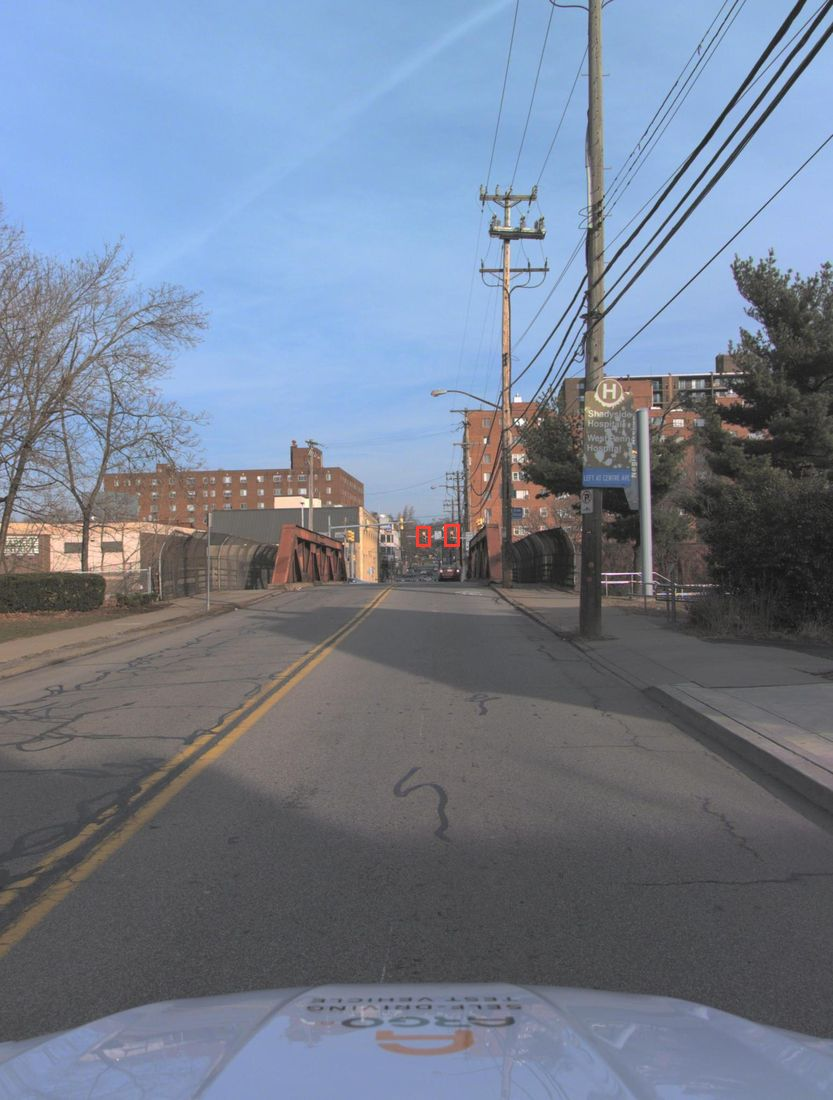
\includegraphics[width=\textwidth]{example_A-0004.jpg}
  \caption{Subset A (Argoverse 2)}
\end{subfigure}\hfill
\begin{subfigure}[b]{0.6\textwidth}
  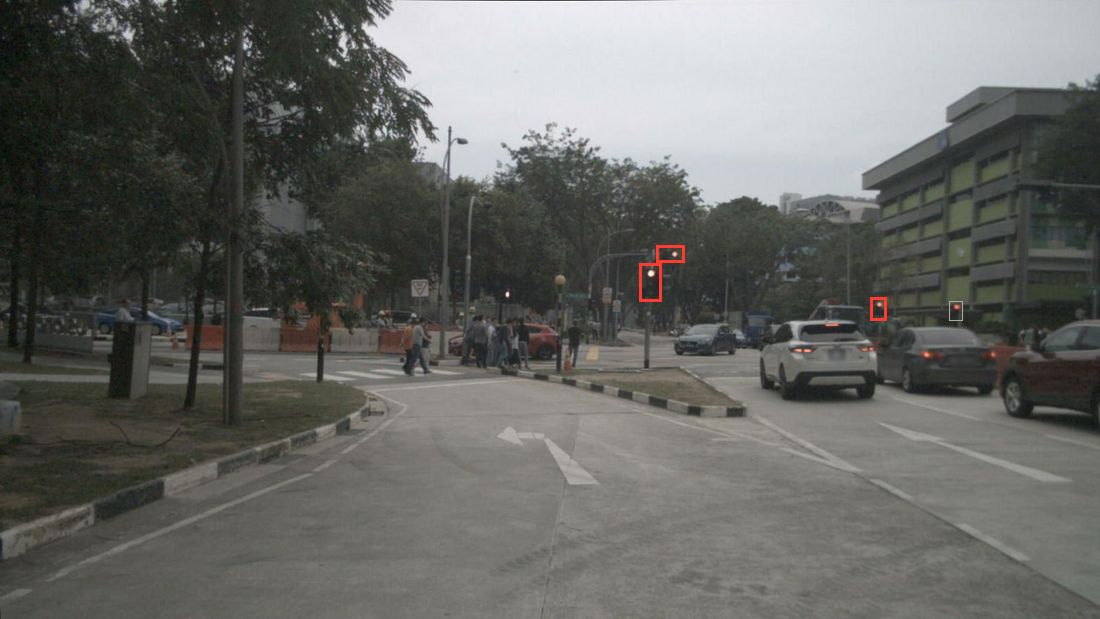
\includegraphics[width=\textwidth]{example_B-0028.jpg}
  \caption{Subset B (nuScenes, Singapore)}
\end{subfigure}
\caption{Validation frames with their annotated lights: lights the label builder marks as relevant for
the ego vehicle are outlined in their signal color, all other lights with a thin grey box.}
\label{fig:examples}
\end{figure}

\section{Results: structured model on OpenLane-V2}
\label{sec:res-openlane}

\begin{table}[t]
\centering
\caption{The structured model (RF-DETR-M, epoch 3, threshold 0.20) on OpenLane-V2 validation, over three
directions. The published values of Zou et al.\ are given for orientation only: they are over four
directions (U-turn included) and on the original, unreleased labels.}
\label{tab:openlane}
\small\setlength{\tabcolsep}{4pt}
\begin{tabular}{@{}lcccccc@{}}
\toprule
 & $\acccolor\uparrow$ & $\accpass\uparrow$ & $\EM\uparrow$ & $\TSS\uparrow$ & $\FG\downarrow$ & $\FS\downarrow$ \\
\midrule
Subset A val & 0.9147 & 0.9474 & 0.8351 & 0.8991 & 0.1516 & 0.0267 \\
Subset B val & 0.9306 & 0.9585 & 0.8569 & 0.9153 & 0.1118 & 0.0134 \\
A+B val & 0.9213 & 0.9520 & 0.8441 & 0.9058 & 0.1319 & 0.0215 \\
\midrule
\emph{Zou et al., direction-aware model} & \emph{0.9019} & \emph{0.9356} & \emph{0.8031} & \emph{0.8802} & \emph{0.1372} & \emph{0.0416} \\
\bottomrule
\end{tabular}
\end{table}

\Cref{tab:openlane} gives the overall result. On subset A val the structured model reaches a TSS of
0.899, and 0.915 on subset B, which is easier on every metric. The numbers lie in the range that Zou et
al.\ report for their direction-aware model (0.880 on their Subset-A), but the two are not directly
comparable: the labels are reconstructed, the number of kept frames differs (\cref{tab:kept-frames}),
and the paper's values include the U-turn. The per-epoch results (\cref{tab:rfdetr-epochs}) vary by about
one TSS point.

\paragraph{Per direction.} The original paper reports no per-direction results. \Cref{tab:perdir-A} and
\cref{fig:perdir} break the subset A results down by maneuver.

\begin{table}[t]
\centering
\caption{Per-direction results of the structured model on subset A val (2,220 frames). GT mix lists
none/red/yellow/green in \%. ``Maj.'' is the color accuracy of always predicting the most frequent color.}
\label{tab:perdir-A}
\small\setlength{\tabcolsep}{3pt}
\begin{tabular}{@{}lccccrc@{}}
\toprule
Direction & GT mix (\%) & $\acccolor$ & $\accpass$ & $\FG$ & \#stop & Maj. \\
\midrule
straight & 3.9 / 28.6 / 5.0 / 62.5 & 0.873 & 0.929 & 0.129 & 636 & 0.625 \\
left & 0.9 / 32.8 / 4.1 / 62.2 & 0.892 & 0.921 & 0.162 & 729 & 0.622 \\
right & 97.7 / 0.6 / 0.1 / 1.5 & 0.979 & 0.992 & 0.643 & 14 & 0.977 \\
\bottomrule
\end{tabular}
\end{table}

\begin{figure}[t]
\centering
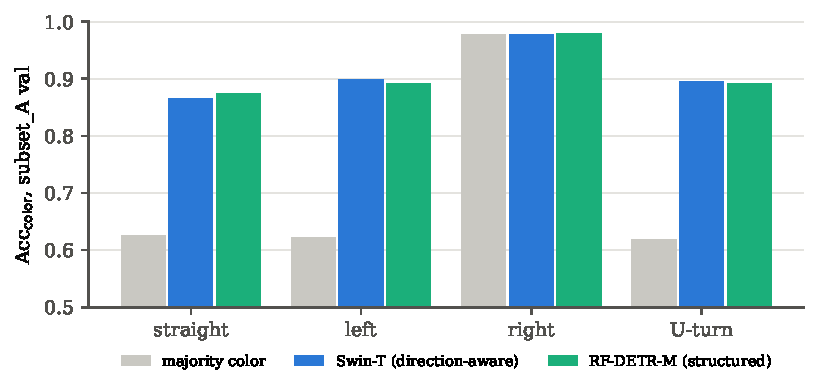
\includegraphics[width=0.85\textwidth]{per_direction.pdf}
\caption{Color accuracy per direction on subset A val, compared with the majority-color baseline.}
\label{fig:perdir}
\end{figure}

\paragraph{Straight and left are learned well.} Their color accuracy is well above the majority
baseline (25 and 27 points on subset A). Straight is the harder of the two on subset A (0.873). Its
\emph{none} class---no light governs straight, as at T-junctions or in turn-only lanes---is rarely
recognized: recall 0.17 on A (87 frames) and 0.46 on B (48 frames).

\paragraph{The right turn is not learned.} Its color accuracy equals the majority baseline (A: 0.979 vs
0.977; B: 0.950 vs 0.958): the model predicts \emph{none} almost always. The few red right-turn signals
(14 frames in A val, 37 in B val) are mostly missed, giving a right-turn False-Go of 0.64 on A and 0.84
on B. These cases are too few to affect the pooled False-Go, yet they are exactly the situations in
which a right turn is forbidden. Zou et al.'s label distribution has the same imbalance (right
\emph{none} 96.9\%), so this is a property of the data rather than of the model.

\paragraph{Yellow is weak on subset A.} Straight yellow recall is 0.53 on A (110 frames) against 0.68 on
B (34 frames); yellow is mostly confused with red or green. Since A has more yellow examples than B, this
is not only a sample-size effect; the amber rendering of Argoverse~2's camera, which makes yellow lamps
resemble red ones, is a likely contributor.

\paragraph{Passability follows color.} In the structured pipeline the passability is derived from the
color by the rule, so the two are consistent by construction, and all go/stop errors stem from color
errors, mainly red confused with green or yellow.

\section{Results: training and testing on DTLD}
\label{sec:res-dtld}

\begin{figure}[t]
\centering
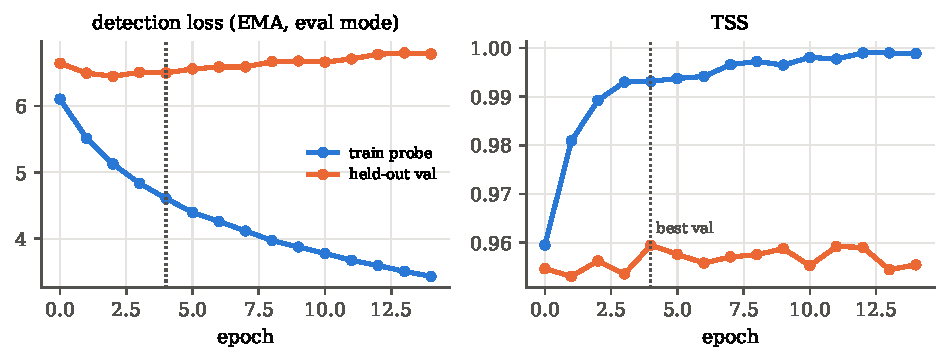
\includegraphics[width=\textwidth]{dtld_overfitting.pdf}
\caption{Overfitting report of the RF-DETR model trained on DTLD: detection loss and TSS on a fixed
probe of the training data and on the held-out tune split. The dotted line marks the best tune epoch.
TSS over four directions, as computed during training for the epoch selection.}
\label{fig:dtld-overfit}
\end{figure}

Trained on DTLD's fit split, the structured model reaches its best tune TSS of 0.9595 (four directions)
at epoch~4
(\cref{fig:dtld-overfit}). Afterwards the model overfits: the probe loss keeps falling (from 4.61 at
epoch 4 to 3.43 at epoch 14) and the probe TSS approaches 1.0, while the tune loss rises (6.50 to 6.79)
and the tune TSS stops improving. About five epochs are therefore sufficient.

\begin{table}[t]
\centering
\caption{RF-DETR-M on DTLD test (11,347 frames, German right-turn rule).}
\label{tab:dtld}
\small
\begin{tabular}{@{}lcccccc@{}}
\toprule
 & $\acccolor$ & $\accpass$ & $\EM$ & $\TSS$ & $\FG$ & $\FS$ \\
\midrule
Epoch 4 (best tune), thr.\ 0.25 & 0.966 & 0.979 & 0.928 & 0.958 & 0.034 & 0.015 \\
Epoch 14 (last), thr.\ 0.30 & 0.966 & 0.978 & 0.928 & 0.958 & 0.032 & 0.017 \\
\midrule
\multicolumn{7}{@{}l}{\emph{Per direction, epoch 14 ($\acccolor$ / $\accpass$ / $\FG$ / majority)}} \\
straight & \multicolumn{6}{l}{0.974 / 0.983 / 0.030 / 0.654} \\
left & \multicolumn{6}{l}{0.975 / 0.980 / 0.021 / 0.571} \\
right & \multicolumn{6}{l}{0.948 / 0.973 / 0.050 / 0.617} \\
\bottomrule
\end{tabular}
\end{table}

On DTLD test (\cref{tab:dtld}) the model reaches a TSS of 0.958 with a False-Go rate of only 0.034, far
lower than on OpenLane-V2. Under German rules right is no longer trivial (majority accuracy 0.617, with
3,231 stop labels), and it is the weakest direction (color accuracy 0.948), but it is clearly learned:
its False-Go rate is 0.050, against 0.64--0.89 for the rare right-turn reds of OpenLane-V2. Overfitting
after epoch 4 costs nothing on test: the last epoch gives the same TSS. Inference takes 22\,ms per frame
on the RTX~5070 (bf16, batch 1), or 37\,ms including JPEG decoding and resizing.

Why DTLD is so much easier than OpenLane-V2 cannot be settled with the experiments at hand. Plausible
contributors are that its relevance is derived from the route actually driven rather than from a lane
graph, that the training set is larger and drawn from a single camera setup, and that its 2:1 images lose
less resolution when resized to the square input than the portrait Argoverse~2 images do. The labels are
also built by different rules, so the two scores measure related but not identical tasks.

\section{Results: out-of-distribution evaluation}
\label{sec:res-ood}

The DTLD model (epoch 4, threshold 0.25) was evaluated without any retraining on LISA test and on
OpenLane-V2 validation, both under the US right-turn rule. \Cref{tab:ood} summarizes the results.

\begin{table}[t]
\centering
\caption{Out-of-distribution results of the DTLD-trained RF-DETR model (source threshold 0.25, images
squeezed to the square input). ``no right'' excludes the right direction. In-domain references: DTLD test
TSS 0.958; RF-DETR trained on OpenLane-V2: A 0.899, B 0.915.}
\label{tab:ood}
\small\setlength{\tabcolsep}{4pt}
\begin{tabular}{@{}lrcccccc@{}}
\toprule
Target & frames & $\TSS$ & $\TSS$ no right & $\acccolor$ & $\EM$ & $\FG$ & $\FS$ \\
\midrule
LISA test & 17,612 & 0.916 & 0.900 & 0.892$^\ast$ & 0.863 & 0.041$^\ast$ & 0.078$^\ast$ \\
\quad day & 7,306 & -- & 0.952 & & & & \\
\quad night & 10,306 & -- & 0.863 & & & & \\
OpenLane-V2 A val & 2,219 & 0.875 & 0.850 & 0.889 & 0.813 & 0.331 & 0.010 \\
OpenLane-V2 B val & 1,565 & 0.887 & 0.885 & 0.908 & 0.824 & 0.177 & 0.031 \\
\bottomrule
\multicolumn{8}{@{}l}{\footnotesize $^\ast$ without the right direction (always \emph{none} on LISA).}
\end{tabular}
\end{table}

\paragraph{LISA.} By day the model transfers well: a no-right TSS of 0.952 is close to its in-domain
DTLD performance, despite a different country and camera. At night the TSS drops to 0.863. Unlike on
OpenLane-V2, errors lean towards False-Stop (0.078) rather than False-Go (0.041). Since a missed light
leaves a maneuver at \emph{none}, which means \emph{go}, False-Stop errors come from lights read as red
that are not; at night, tail lights and other red light sources are plausible confusers. Neither
re-tuning the threshold on LISA's own tune split (no-right TSS 0.868) nor padding the images to the 2:1
training aspect (0.865) closes the gap, so it is not a calibration or geometry issue.

\paragraph{OpenLane-V2.} On nuScenes images (subset B) the DTLD model reaches a TSS of 0.887, three points
below the model trained in-domain (0.915). On Argoverse~2 images (subset A) the TSS drop is similar
(0.875 vs 0.899), but the False-Go rate more than doubles (0.331 vs 0.152): the model frequently declares
straight (False-Go 0.29) and left (0.35) maneuvers free when their signal is red. In the structured
pipeline a relevant light that is not detected leaves its maneuver at \emph{none}, that is, \emph{go}, so
missed red lights turn directly into False-Go errors. Two effects plausibly combine to cause the misses: the amber, red-leaning color rendering of the Argoverse~2 camera that already made yellow
hard in-domain, and the portrait geometry, which after squeezing into a square makes lights appear at a
different aspect ratio than in the wide DTLD images. Padding the portrait images to 2:1 instead makes
the lights even smaller and the results much worse (TSS 0.804, False-Go 0.48); threshold re-tuning
changes the results by less than half a point.

\section{Results: per-light evaluation on ATLAS}
\label{sec:res-atlas}

ATLAS has no relevance or maneuver labels, so the DTLD model is evaluated per light: each annotated light
is matched to the detections (class-agnostic, greedy by score, IoU $\ge$ 0.5), and detection recall and
precision, color accuracy on matched lights and, for arrows, whether the predicted maneuver set equals
the arrow's direction are measured. The evaluation uses the official ATLAS test
split of each camera; lights that are off are not among the model's classes and are not counted.

\begin{table}[t]
\centering
\caption{Per-light results of the DTLD-trained model on the three ATLAS cameras (IoU 0.5; in brackets
IoU 0.3).}
\label{tab:atlas}
\small
\begin{tabular}{@{}lrrcccc@{}}
\toprule
Camera & images & lights & recall & precision & color acc. & arrow moves acc. \\
\midrule
wide & 828 & 2,055 & 0.469 (0.585) & 0.569 (0.723) & 0.962 & 0.436 \\
medium & 1,003 & 2,064 & 0.658 (0.729) & 0.644 (0.731) & 0.887 & 0.468 \\
tele & 997 & 2,050 & 0.679 (0.759) & 0.606 (0.698) & 0.895 & 0.481 \\
\bottomrule
\end{tabular}
\end{table}

\begin{figure}[t]
\centering
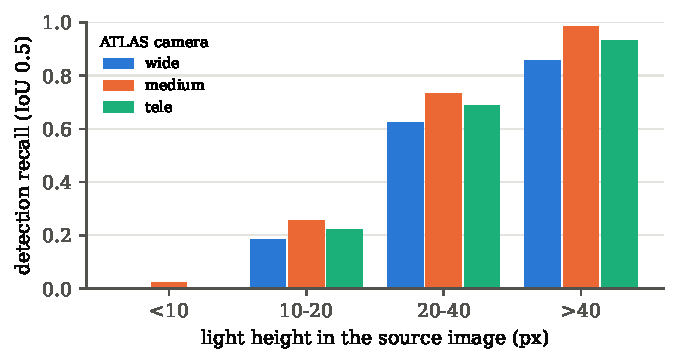
\includegraphics[width=0.75\textwidth]{atlas_recall.pdf}
\caption{Detection recall on ATLAS as a function of the light's height in the source image.}
\label{fig:atlas}
\end{figure}

\Cref{tab:atlas} and \cref{fig:atlas} show that detection is the bottleneck. Recall depends almost
entirely on the light's size: lights taller than 40 pixels are found in 86--98\% of the cases, lights of
20--40 pixels in 62--73\%, lights of 10--20 pixels in only about 20\%, and lights below 10 pixels
practically never. The wide camera, whose lights are smallest, has the lowest recall. The much higher
recall at IoU 0.3 indicates that a part of the misses are localization errors on small boxes rather than
missed lights. Color, once a light is detected, is recognized with 89--96\% accuracy. The arrow result is
the weakest: for fewer than half of the matched arrows does the predicted maneuver set equal the arrow's
direction. Part of this is by design: the model's classes encode the maneuvers a light controls for the ego
vehicle, as derived from the DTLD route labels, not the pictogram as such, so an arrow can legitimately
receive a broader class such as the one used for circles. Even so, the result shows that the model does
not reliably carry over pictogram recognition to a new camera setup.

\section{Computational cost}
\label{sec:res-cost}

\Cref{tab:cost} collects the cost of the models trained in this work.

\begin{table}[t]
\centering
\caption{Model size and training cost on one RTX 5070.}
\label{tab:cost}
\small
\begin{tabular}{@{}lrrll@{}}
\toprule
Model & Params & Epochs & Time / epoch & Peak mem. \\
\midrule
RF-DETR-M, OpenLane-V2 & 34.6M & 4 & $\approx$20 min & 6.5 GiB \\
RF-DETR-M, DTLD & 34.6M & 15 & $\approx$27 min & 6.6 GiB \\
\bottomrule
\multicolumn{5}{@{}l}{\footnotesize Time per epoch including validation.} \\
\end{tabular}
\end{table}

A few epochs of fine-tuning suffice on both datasets, and at inference the model runs at 22\,ms per
frame (\cref{sec:res-dtld}), comfortably within the frame rate of automotive cameras.

\chapter{Discussion and Future Perspectives}
\label{ch:discussion}

This chapter interprets the results of \cref{ch:method}. It compares them with the original paper and
the wider literature (\cref{sec:disc-compare}), discusses their theoretical and practical implications
(\cref{sec:disc-implications}), states the limitations of the work (\cref{sec:disc-limits}) and proposes
directions for future research (\cref{sec:disc-future}).

\section{Comparison with previous work}
\label{sec:disc-compare}

\paragraph{Confirmations.} The label semantics of Zou et al.\ can be recovered from the public
annotations. That the reconstructed label distribution matches the paper's Fig.~3 for almost every
class suggests that the specificity hierarchy, left inheriting straight and right governed only by
dedicated signals were rebuilt correctly. A model trained on these labels reaches a TSS of 0.899 on
subset A val, in the range the paper reports for its direction-aware model (0.880). This confirms that
maneuver-level prediction from a single image is feasible without HD maps, which map-based
systems~\cite{fairfield2011traffic,possatti2019traffic,polley2025atlas} rely on, and without the
annotated lane metadata of earlier map-free work~\cite{langenberg2019deep}.

\paragraph{Differences.} The rebuilt benchmark contains about 29\% fewer frames than the paper's, for
reasons that cannot be determined without the original filtering rules. The paper describes its data as
Subset-A, which its own frame counts contradict; the evidence collected here (frame counts, color mix,
right-turn distribution under US rules) points to A+B. A further difference is deliberate: the results
here are over three maneuvers, without the U-turn, which follows the left signal in 99.9\% of the labels.
For these reasons the scores of this thesis and the published ones are close in scale but are not a
head-to-head comparison.

\paragraph{Structured pipelines.} The original paper reports that its direction-aware model clearly
outperforms structured pipelines. Its strongest structured baseline, TLD-READY~\cite{polley2024tldready},
was designed for per-light relevance on German roads and adapted to the four-maneuver output with a
fallback to the circular signal; it reaches a TSS of 0.842 and a False-Go rate of 0.302. The structured
model of this thesis reaches 0.899 and 0.152 on subset A val, because its classes encode the maneuvers
each light controls and therefore mirror the label rules exactly, so that a perfect detector would be a
perfect predictor. Allowing for the differences in labels and directions, this suggests that the gap
reported in the paper reflects the design of the structured baselines it used rather than an inherent
limit of the structured approach. This is in line with the broader experience in detection that
well-tuned, strongly pretrained detectors~\cite{zhao2024detrs,chen2024lwdetr,robinson2025rfdetr} are hard
to beat.

\section{Theoretical and practical implications}
\label{sec:disc-implications}

\paragraph{Aggregate scores hide the safety-critical cases.} The right-turn analysis shows that a model
can reach state-of-the-art TSS while failing on nearly every forbidden right turn, because these cases
are rare and pooled metrics weight them by frequency. The same holds, to a lesser degree, for yellow and
for straight \emph{none}. Benchmarks for this task should therefore report per-direction results,
class-wise recall of the rare states and, ideally, a False-Go rate per maneuver. The TSS, which weighs
False-Go and False-Stop equally and lets the trivial right direction contribute a quarter of the
accuracies, is a poor proxy for safety on its own.

\paragraph{Label conventions are part of the model.} The meaning of a right-turn label differs between
the US and Germany, and the choice of convention changes the right-turn distribution from 97\% \emph{none}
to 63\% green. An end-to-end model internalizes whichever convention it is trained on. A structured
pipeline can change the rule at inference time, which is a practical argument for keeping the traffic
rules explicit, especially for systems meant to operate in more than one country.

\paragraph{Detection is the bottleneck out of distribution.} The ATLAS results show that most errors of a
transferred model begin with lights that are not detected, and that detection depends steeply on light
size. In the structured pipeline, a missed red light becomes a \emph{go} decision by default, which
explains the high False-Go on Argoverse~2 images. A safer design would treat ``no relevant light
found'' near an intersection as uncertain rather than as permission, as the map-based ATLAS framework
does by mapping an unknown signal-group state to red~\cite{polley2025atlas}. The same work shows that a
tele camera and a wide-angle camera are the practical answer to the size problem, and that a detector
trained on DTLD alone is clearly weaker on ATLAS images than one that also saw ATLAS data (mAP@50 about
0.53 versus 0.7); the per-light results obtained
here with a different detector point the same way. Trinci et al.~\cite{trinci2026color} likewise found
that relevance models do not transfer between DTLD and US data, so the transfer gaps measured in this
thesis appear to be a property of the data rather than of a particular architecture.

\paragraph{Cost and deployability.} The structured model runs at 22\,ms per frame on a consumer GPU and
needs only a few epochs of fine-tuning, which makes it a realistic component for an embedded perception
stack. Its explicit intermediate output (which lights were found and what they control) also supports
monitoring and debugging, an important property for safety arguments.

\section{Limitations}
\label{sec:disc-limits}

\begin{itemize}
  \item \textbf{Reconstructed labels.} The benchmark is a reconstruction. Its rules were validated against
        the published distribution and by spot-checking about 80 frames across datasets, but no full
        manual quality control was done. Some label noise certainly remains, and the left~$=$~none
        mismatch shows a systematic difference from the original.
  \item \textbf{Single seeds.} Each configuration was trained once. The epoch-to-epoch variation of the
        OpenLane-V2 model (about one TSS point, \cref{tab:rfdetr-epochs}) is of the same order as the
        differences one would want to resolve, so conclusions about small differences are limited.
  \item \textbf{Evaluation on the validation split.} OpenLane-V2's test split has no usable annotations,
        so, as in the original paper, the validation split is the evaluation set. Model selection was
        kept away from it, but it is still a split that has been looked at during development.
  \item \textbf{No head-to-head comparison with the original model.} Neither the original labels nor
        its code are public, so the published numbers can only be set beside the results of this thesis
        with the caveats of \cref{sec:disc-compare}. The structured model's class encoding is, moreover,
        tailored to the label rules.
  \item \textbf{Size-based relevance on LISA.} LISA has no relevance labels, so the ego intersection's
        lights were identified by their size. Trinci et al.~\cite{trinci2026color} show that the
        largest light is a poor relevance cue in the United States; the LISA labels are therefore
        noisier than those of OpenLane-V2 and DTLD, and the LISA results should be read as an
        approximate measure of transfer.
  \item \textbf{Convention mismatch in Singapore.} For comparability, US rules were applied to left-hand
        traffic scenes, which is semantically incorrect for those frames.
  \item \textbf{Single frames.} All models see one image. Flashing signals, occlusions and the short
        yellow phase cannot be resolved reliably without temporal context.
\end{itemize}

\section{Future research directions}
\label{sec:disc-future}

\begin{itemize}
  \item \textbf{Safety-oriented training and evaluation.} Class-balanced or cost-sensitive losses that
        penalize False-Go more than False-Stop, and benchmark protocols with per-direction and
        per-class reporting, would align optimization with the actual risk.
  \item \textbf{Rule-aware models.} Conditioning the model on the applicable traffic convention (country,
        left- or right-hand traffic), or keeping the rules explicit as in the structured pipeline, would
        let a single model operate across jurisdictions and label the Singapore scenes correctly.
  \item \textbf{Temporal models.} Aggregating evidence over a short sequence would stabilize predictions,
        handle occlusions, and allow flashing and phase-change states to be modeled.
  \item \textbf{Multi-dataset training.} The DTLD and LISA labels built here use compatible conventions,
        so mixed training across countries and illumination conditions is the natural next experiment,
        with LISA's night sequences as the main robustness test. ATLAS, BSTLD, S$^2$TLD and BDD100K
        could add pictograms, cameras, weather and countries to the detector's training data, and
        VZC-TLD, the only US dataset with relevance labels, would allow an image-level test of the
        stop/go decision outside Germany.
  \item \textbf{Small-object detection.} Higher input resolution around the horizon, tiled inference or
        a dedicated tele camera (as on ATLAS) target the steepest failure mode observed here.
  \item \textbf{Uncertainty.} Calibrated confidence for each maneuver, and an explicit ``unknown'' output
        when no relevant light is found at an approaching intersection, would allow a planner to act
        conservatively instead of defaulting to \emph{go}.
  \item \textbf{Fusion with maps and topology.} Where maps or online topology
        predictions~\cite{li2023graph,wu2024topomlp} are available, they could supply the relevance that
        single-image models must currently infer.
\end{itemize}

\chapter*{Conclusions}
\addcontentsline{toc}{chapter}{Conclusions}
\markboth{Conclusions}{Conclusions}

This thesis set out to examine a simple but demanding idea: that a vehicle can decide from one camera
image, without a map, whether each of its possible maneuvers at the next intersection is permitted by
the traffic signals. The main objective was to establish, independently and from public data only, how
well current models solve this task, what their accuracy depends on, and how far it carries beyond the
data they were trained on.

\paragraph{Answers to the research questions.}
\begin{description}[leftmargin=1.2cm,style=nextline]
  \item[RQ1] \emph{Benchmark reconstruction.} Yes. Labels rebuilt from the OpenLane-V2 lane and
        traffic-element topology reproduce the published per-direction label distribution for almost
        every class, with one systematic difference (left \emph{none}). The evidence also indicates that
        the original benchmark combines subsets A and B under US rules, rather than subset A alone as
        stated.
  \item[RQ2] \emph{Structured model.} A structured pipeline---an RF-DETR detector whose classes encode
        the maneuvers each light controls, followed by explicit rules---reaches a TSS of 0.899 on subset A
        and 0.915 on subset B, in the range published for the end-to-end direction-aware model, although
        the two are not directly comparable. It fails where the data are thin: right-turn reds, yellow,
        and straight maneuvers that no light governs.
  \item[RQ3] \emph{Transfer.} A model trained on German data (DTLD, test TSS 0.958) transfers well to US
        day-time driving (LISA day 0.952 without right turns) but loses ten points at night and doubles
        its False-Go rate on Argoverse~2 images. Detection of small lights is the dominant failure: on
        ATLAS, recall falls from over 85\% for lights taller than 40 pixels to about 20\% for lights of
        10--20 pixels.
\end{description}

\paragraph{What emerged from the analysis.} Beyond the individual numbers, the work points to three
broader lessons. First, aggregate scores conceal the decisions that matter most: models with
state-of-the-art TSS miss almost every red right-turn arrow, and yellow lights and straight maneuvers
without a governing signal are weak points as well. Second, traffic rules are not a detail of the
labels but part of the task's definition; the same image calls for different decisions in the United
States and in Germany, and a design that keeps the rules explicit can adapt to this, where an end-to-end
model has to be relabeled and retrained. Third, in the structured pipeline an undetected light silently becomes a \emph{go}
decision, so robustness out of distribution is above all a question of detecting small, distant lights
and of treating their absence as uncertainty rather than permission.

\paragraph{Limitations.} The conclusions rest on reconstructed labels without full manual quality
control, on single training runs per configuration, on evaluation with the validation split of
OpenLane-V2, and on single-frame models. Small differences between models are therefore reported as
non-significant rather than as rankings.

\paragraph{Future developments.} The most promising continuations are safety-weighted training and
evaluation protocols that report per-maneuver False-Go rates, models conditioned on the applicable
traffic convention, temporal aggregation over short sequences, training on mixed datasets from several
countries and lighting conditions, and better detection of small lights through resolution or a tele
camera. Together they would move maneuver-level signal understanding from a benchmark score towards a
component whose failures are understood, bounded and acceptable on the road.


\renewcommand{\bibname}{References}
\clearpage\phantomsection
\addcontentsline{toc}{chapter}{References}
\bibliographystyle{unsrtnat}
\bibliography{references}

\chapter*{Web References}
\addcontentsline{toc}{chapter}{Web References}
All pages accessed on 3 November 2026.
{\raggedright
\begin{enumerate}[label={[W\arabic*]},leftmargin=1.4cm,itemsep=4pt]
  \webitem{web:openlanev2} OpenDriveLab. \emph{OpenLane-V2 dataset and devkit}.
        \url{https://github.com/OpenDriveLab/OpenLane-V2}
  \webitem{web:dtld} J.~Müller. \emph{DriveU Traffic Light Dataset (DTLD): parser and access
        instructions}. \url{https://github.com/julimueller/dtld_parsing}
  \webitem{web:lisa} Laboratory for Intelligent and Safe Automobiles, UC San Diego. \emph{LISA Traffic
        Light Dataset}. \url{https://www.kaggle.com/datasets/mbornoe/lisa-traffic-light-dataset}
  \webitem{web:atlas} FZI Research Center for Information Technology. \emph{ATLAS: Applied Traffic
        Light Annotation Set}. \url{https://url.fzi.de/ATLAS}
  \webitem{web:bstld} Bosch. \emph{Bosch Small Traffic Lights Dataset}.
        \url{https://hci.iwr.uni-heidelberg.de/content/bosch-small-traffic-lights-dataset}
        \todo{check URL}
  \webitem{web:s2tld} Thinklab, Shanghai Jiao Tong University. \emph{S$^2$TLD: SJTU Small Traffic
        Light Dataset}. \url{https://github.com/Thinklab-SJTU/S2TLD}
  \webitem{web:vzc} Verizon Connect Research. \emph{VZC-TLD: Verizon Connect Traffic Light Dataset}.
        \url{https://leotac.github.io/vzc-tld}; data:
        \url{https://huggingface.co/datasets/vzc-research-chapter/vzc-traffic-light-dataset}
  \webitem{web:bdd100k} Berkeley DeepDrive. \emph{BDD100K dataset}. \url{https://bdd-data.berkeley.edu}
  \webitem{web:tldready} KASTEL Mobility Lab. \emph{TLD-READY: code, model weights and relevance
        labels}. \url{https://github.com/KASTEL-MobilityLab/traffic-light-detection}
  \webitem{web:pytorch} PyTorch Foundation. \emph{PyTorch}. \url{https://pytorch.org}
  \webitem{web:rfdetr} Roboflow. \emph{RF-DETR: real-time object detection and segmentation}.
        \url{https://github.com/roboflow/rf-detr}\end{enumerate}
\par}

\appendix
\chapter{Label Construction Rules}
\label{app:labels}

\section{OpenLane-V2}

The label builder (\code{dtsu/labels.py}) processes each frame as follows.

\begin{enumerate}
  \item \textbf{Traffic elements.} Read the front-image traffic elements and their attribute: 1 red,
        2 green, 3 yellow for circular lights; 4--12 for arrow types (left, right, straight, U-turn and
        their combinations).
  \item \textbf{Ego approach lanes.} Select lane centerlines that start ahead of the ego vehicle and are
        aligned with its heading (within $60^\circ$).
  \item \textbf{Maneuver per lane.} From each approach lane, follow \code{topology_lclc} to the first
        junction lane being entered; the entering lane may start up to 3\,m behind the ego vehicle
        (\code{ENTERING_X = -3 m}). Classify the heading change along that lane: $|\Delta\psi|\le30^\circ$
        straight, $|\Delta\psi|>135^\circ$ U-turn, otherwise left or right by the sign of $\Delta\psi$.
  \item \textbf{Relevant lights.} Through \code{topology_lcte}, collect the lights linked to the selected
        lanes of the nearest junction (within 10\,m). If the ego vehicle has passed the stop line, use
        approach lanes ending within 30\,m behind it.
  \item \textbf{Assignment.} For each relevant light, record the set of maneuvers it controls. Then:
        straight $\leftarrow$ straight-specific or generic lights; left $\leftarrow$ left-specific lights,
        else straight; U-turn $\leftarrow$ U-turn-specific lights, else left; right $\leftarrow$ lights
        that control only the right turn, else \emph{none}. Among candidates, the most specific light
        (fewest controlled maneuvers) wins.
  \item \textbf{Conflicts and filter.} Equally specific candidates with different colors mark a conflict
        and drop the frame. Frames without any relevant colored light are dropped.
  \item \textbf{Traffic side.} US (right-hand) rules are applied to all frames, including Singapore. A
        mirrored variant for left-hand traffic is kept for analysis only.
\end{enumerate}
Each record stores the image path, the four colors and passabilities, the traffic side, the
right-turn convention (\code{near_turn}) and all light boxes with their controlled maneuvers and a
relevance flag (used by the structured baseline).

\section{DTLD}

\begin{enumerate}
  \item Consider front-facing vehicle lamps (circles and arrows); pedestrian and other lamps are
        ignored.
  \item The ego intersection's lamps are the relevant ones plus non-relevant lamps at least 0.6 times
        the median height of the relevant ones.
  \item A route with its own arrow (left, right, straight, straight-left) is served by that arrow; a
        route without an arrow is served by the circles.
  \item States: red and red--yellow $\to$ red, yellow $\to$ yellow, green $\to$ green; off or unknown
        lamps give no color, and a direction whose lamps all lack one drops the frame.
  \item Directions: straight, left and right take their lamps' colors; left without lamps inherits
        straight; U-turn inherits left (DTLD has no U-turn signals). Right uses the German convention
        (\code{near_turn = "signal"}).
\end{enumerate}

\section{LISA}

\begin{enumerate}
  \item Lights are grouped by kind (circle, left arrow, straight arrow).
  \item A light is at the ego intersection if its height is at least 0.6 times that of the tallest light
        of the same kind in the frame.
  \item Directions follow the OpenLane-V2 rules under the US convention; right is always \emph{none}.
  \item Frames with conflicts or with arrows only are dropped.
\end{enumerate}

\chapter{Hyperparameters}
\label{app:hparams}

\begin{table}[h]
\centering
\caption{Training settings of the direction-aware model.}
\label{tab:hparams-dam}
\small
\begin{tabularx}{\textwidth}{@{}lX@{}}
\toprule
Setting & Value \\
\midrule
Backbone & Swin-T \code{swin_tiny_patch4_window7_224} (ImageNet-1k), LayerNorm per output stage, drop-path 0.1 \\
Neck & FPN, 256 channels, P2--P5 \\
Detector & DETR, 6 encoder layers (P5), 6 decoder layers (P3, P4, encoded P5), 50 queries, 3 classes \\
ROI tokens & $K=16$, RoIAlign on P2, $7\times7$ \\
Direction attention & 4 queries, 8 heads, 1 layer + LayerNorm + FFN \\
Loss & $\lambda_c=1$, $\lambda_p=1$, $\lambda_d=0.2$; DETR: class + $5\,L_1$ + $2\,$GIoU, auxiliary losses \\
Optimizer & AdamW, lr $10^{-4}$ (backbone $10^{-5}$), weight decay $10^{-4}$ \\
Schedule & cosine over 24 epochs, 500 warm-up iterations, stopped after epoch 14 \\
Gradient clipping & 0.1 \\
Batch & 4 (one canvas shape per batch) \\
Input & long side 1024, aspect kept, padded to a multiple of 32 \\
Augmentation & brightness and contrast jitter $[0.75, 1.25]$; no flips, no hue shift \\
Precision & fp16 backbone/FPN, bf16 detector, fp32 ROI/direction branch, TF32 \\
\bottomrule
\end{tabularx}
\end{table}

\begin{table}[h]
\centering
\caption{Training settings of the structured RF-DETR baseline.}
\label{tab:hparams-rfdetr}
\small
\begin{tabularx}{\textwidth}{@{}lX@{}}
\toprule
Setting & Value \\
\midrule
Model & RF-DETR Medium, 34.6M parameters, fine-tuned from the released weights \\
Classes & \code{<moves>|<color>}: 46 (OpenLane-V2 A+B), 24 (DTLD) \\
Resolution & 1024$\times$1024 square resize, no multi-scale, no scale jitter \\
Augmentation & brightness and contrast jitter; no flips, no crops \\
Optimizer & library default; lr $10^{-4}$, encoder lr $1.5\cdot10^{-4}$, EMA weights evaluated \\
Batch & 4, gradient accumulation 4 \\
Epochs & 4 (OpenLane-V2), 15 with per-epoch report (DTLD) \\
Inference & score threshold 0.20 (OpenLane-V2, from tuning), 0.25 (DTLD, from tune split); class-agnostic NMS at IoU 0.5 \\
\bottomrule
\end{tabularx}
\end{table}

\chapter{Per-Epoch Results}
\label{app:epochs}

\begin{table}[h]
\centering
\caption{TSS per epoch on subset A, subset B and A+B val, direction-aware model with both backbones, and
subset A False-Go.}
\label{tab:epochs}
\small
\begin{tabular}{@{}r cccc cccc@{}}
\toprule
 & \multicolumn{4}{c}{Swin-T} & \multicolumn{4}{c}{ConvNeXtV2-T} \\
\cmidrule(lr){2-5}\cmidrule(lr){6-9}
Epoch & A & B & A+B & $\FG_A$ & A & B & A+B & $\FG_A$ \\
\midrule
0 & 0.891 & 0.910 & 0.899 & 0.124 & 0.863 & 0.886 & 0.872 & 0.169 \\
1 & 0.893 & 0.895 & 0.894 & 0.182 & 0.875 & 0.904 & 0.887 & 0.181 \\
2 & 0.888 & 0.925 & 0.903 & 0.223 & 0.890 & 0.916 & 0.900 & 0.150 \\
3 & 0.896 & 0.927 & 0.909 & 0.145 & 0.886 & 0.908 & 0.895 & 0.228 \\
4 & 0.904 & 0.928 & 0.914 & 0.107 & 0.884 & 0.908 & 0.894 & 0.183 \\
5 & 0.899 & 0.936 & 0.914 & 0.170 & 0.895 & 0.922 & 0.906 & 0.192 \\
6 & 0.899 & 0.926 & 0.910 & 0.139 & 0.890 & 0.905 & 0.896 & 0.222 \\
7 & 0.904 & 0.937 & 0.918 & 0.112 & 0.893 & 0.900 & 0.896 & 0.204 \\
8 & 0.899 & 0.928 & 0.911 & 0.105 & 0.896 & 0.928 & 0.909 & 0.174 \\
9 & 0.893 & 0.912 & 0.901 & 0.189 & 0.884 & 0.919 & 0.898 & 0.241 \\
10 & 0.908 & 0.927 & 0.916 & 0.132 & 0.892 & 0.914 & 0.901 & 0.186 \\
11 & 0.887 & 0.891 & 0.889 & 0.212 & 0.879 & 0.912 & 0.893 & 0.209 \\
12 & 0.903 & 0.920 & 0.910 & 0.135 & 0.891 & 0.910 & 0.899 & 0.188 \\
13 & 0.897 & 0.912 & 0.903 & 0.141 & 0.905 & 0.932 & 0.916 & 0.112 \\
14 & 0.889 & 0.911 & 0.898 & 0.164 & 0.894 & 0.919 & 0.905 & 0.194 \\
\bottomrule
\end{tabular}
\end{table}

\begin{table}[h]
\centering
\caption{RF-DETR-M on OpenLane-V2 val per epoch (threshold 0.20). The reported model is epoch 3.}
\label{tab:rfdetr-epochs}
\small
\begin{tabular}{@{}rccccc@{}}
\toprule
Epoch & TSS A & TSS B & TSS A+B & $\FG$ A+B & $\FS$ A+B \\
\midrule
0 & 0.909 & 0.919 & 0.913 & 0.113 & 0.029 \\
1 & 0.900 & 0.919 & 0.908 & 0.133 & 0.025 \\
2 & 0.902 & 0.913 & 0.907 & 0.135 & 0.021 \\
3 & 0.895 & 0.914 & 0.903 & 0.130 & 0.024 \\
\bottomrule
\end{tabular}
\end{table}

\chapter{Reproducing the Results}
\label{app:repro}

All commands run from the repository root. Data paths assume OpenLane-V2 under
\code{data/OpenLane-V2/} and DTLD, LISA and ATLAS under the directory given by the \code{DATASETS}
environment variable.

\begin{lstlisting}
# OpenLane-V2 labels (per subset and split)
python -m dtsu.labels --root data/OpenLane-V2/subset_A --split train \
  --data-dict data/OpenLane-V2/subset_A/data_dict_subset_A.json \
  --out data/labels/subset_A_train.jsonl
# DTLD and LISA labels, fit/tune splits
bash tools/build_ext_labels.sh
# unit tests (labels, metrics)
python -m pytest tests
# direction-aware model, Swin-T (resumable) and per-direction evaluation
bash tools/run_full.sh
python tools/eval_directions.py
# backbone ablation
bash tools/run_convnextv2.sh
# RF-DETR: tuning, final OpenLane-V2 run, DTLD run
bash tools/run_rfdetr_tuning.sh
bash tools/run_rfdetr.sh
bash tools/run_rfdetr_dtld.sh
# paired segment-level bootstrap
python tools/bootstrap_compare.py
# out-of-distribution evaluation of the DTLD model
python tools/eval_rfdetr_ood.py --target lisa --epoch 4 --source-threshold 0.25
python tools/eval_rfdetr_ood.py --target openlane --epoch 4 --source-threshold 0.25
python tools/eval_rfdetr_atlas.py --epoch 4 --threshold 0.25
# figures of this thesis
python thesis/make_figures.py
\end{lstlisting}

The main outputs are:
\begin{itemize}
  \item \code{runs/swin_t_AB/}: checkpoint, final and per-epoch metrics, per-direction results;
  \item \code{runs/convnextv2_t_AB/}: backbone ablation;
  \item \code{runs/rfdetr_m_AB/}, \code{runs/rfdetr_m_dtld/}: structured baseline, including
        \code{ood_lisa/}, \code{ood_openlane/} and \code{ood_atlas/};
  \item \code{runs/bootstrap_swin_vs_rfdetr.json}: bootstrap comparison.
\end{itemize}


\end{document}
